% options:
% thesis=B bachelor's thesis
% thesis=M master's thesis
% czech thesis in Czech language
% english thesis in English language
% hidelinks remove colour boxes around hyperlinks

\documentclass[thesis=M,czech]{FITthesis}[2013/05/10]

\usepackage[utf8]{inputenc} % LaTeX source encoded as UTF-8

\usepackage{graphicx} %graphics files inclusion
% \usepackage{amsmath} %advanced maths
% \usepackage{amssymb} %additional math symbols

\usepackage{dirtree} %directory tree visualisation

% % list of acronyms
% \usepackage[acronym,nonumberlist,toc,numberedsection=autolabel]{glossaries}
% \iflanguage{czech}{\renewcommand*{\acronymname}{Seznam pou{\v z}it{\' y}ch zkratek}}{}
% \makeglossaries

\newcommand{\tg}{\mathop{\mathrm{tg}}} %cesky tangens
\newcommand{\cotg}{\mathop{\mathrm{cotg}}} %cesky cotangens

% % % % % % % % % % % % % % % % % % % % % % % % % % % % % % 
% ODTUD DAL VSE ZMENTE
% % % % % % % % % % % % % % % % % % % % % % % % % % % % % % 
\usepackage{listings}
\usepackage{cmap}
\parskip = \baselineskip
\hyphenation{nej-ví-ce}
\hyphenation{dy-na-mic-ké-mu}
\hyphenation{zpra-co-vá-ní}
\hyphenation{po-li-tic-kým}
\hyphenation{na-pří-klad}
\hyphenation{nej-pou-ží-va-něj-ších}
\hyphenation{tak-zvaným}
\hyphenation{ka-te-go-rií}
\hyphenation{cho-vá-ní}
\hyphenation{Veš-ke-ré}
\hyphenation{re-gis-tra-ci}
\hyphenation{po-zi-tiv-ně}
\hyphenation{pou-ží-vá}
\hyphenation{ov-lá-dá-ní}
\hyphenation{u-dě-lo-vá-ní}
\hyphenation{no-vé-mu}
\hyphenation{růz-no-ro-dé}
\hyphenation{Naš-těs-tí}
\hyphenation{ne-pot-vr-ze-ných}
\hyphenation{pot-vr-ze-ných}
\hyphenation{fa-ce-boo-ko-vé}
\hyphenation{vy-kres-lo-vá-ní}
\hyphenation{roz-hra-ním}
\hyphenation{Exi-stu-jí}
\hyphenation{proh-lí-že-če}
\hyphenation{proh-lí-že-čů}
\hyphenation{ope-ra-čním}
\hyphenation{strá-nek}
\hyphenation{cel-ko-vou}
\hyphenation{množ-ství}
\hyphenation{prav-dě-po-dob-ně}
\hyphenation{ho-di-na}
\hyphenation{ta-ko-vým-to}
\hyphenation{stej-né-ho}
\hyphenation{pa-ra-me-tr}
\hyphenation{ex-pe-ri-men-tál-ních}
\hyphenation{mai-lo-vé}
\hyphenation{vy-pl-ně-no-sti}
\hyphenation{vy-zkou-še-ní}
\hyphenation{o-pi-so-vá-ním}
\hyphenation{au-to-ma-tic-kým}
\hyphenation{při-hla-šo-vat}
\hyphenation{ta-bul-ce}
\hyphenation{ja-ký-mi-ko-li}
\hyphenation{e-li-mi-no-vat}
\hyphenation{fa-ce-boo-ko-vé}
\hyphenation{a-pli-ka-ce}
\hyphenation{po-stu-pem}
\hyphenation{mož-nost-mi}
\hyphenation{nej-zná-měj-ší}
\hyphenation{stej-né}
\hyphenation{pro-gra-mech}
\hyphenation{pro-hlí-že-če}
\hyphenation{zá-kaz-ní-ky}
\hyphenation{a-pli-ka-ci}
\hyphenation{O-ra-cle}
\hyphenation{vyh-le-dá-vá-ní}
\hyphenation{pro-hlí-že-če}
\hyphenation{přá-te-lích}
\hyphenation{o-stat-ních}
\hyphenation{pra-vdě-po-dob-ně}
\hyphenation{pro-blé-my}
\hyphenation{ex-pe-ri-ment}
\hyphenation{o-sob-ních}
\hyphenation{níz-ko-ú-rov-ňo-vé}
\hyphenation{Ja-va-Scrip-to-vých}
\hyphenation{spo-leč-nost}
\hyphenation{da-ta-bá-ze}
\hyphenation{slou-ží}
\hyphenation{pře-de-vším}
\hyphenation{vy-hle-dá-vá-ní}
\hyphenation{nej-roz-sáh-lej-ší}
\hyphenation{sy-sté-mem}
\hyphenation{pra-vdě-po-do-bně}
\hyphenation{fy-zic-kých}
\hyphenation{pro-dlu-žo-vat}
\hyphenation{ge-ne-ra-ce}
\hyphenation{ak-tiv-ní}
\hyphenation{po-tvr-ze-ných}
\hyphenation{ne-po-tvr-ze-ných}
\hyphenation{Na-štěs-tí}
\hyphenation{do-stup-ný-mi}
\hyphenation{o-stat-ní}
\hyphenation{Prak-tic-ky}
\hyphenation{ob-ráz-ků}
\hyphenation{prav-dě-po-dob-ně}
\hyphenation{ús-pěš-ném}
\hyphenation{o-me-ze-ně}
\hyphenation{růz-ných}
\hyphenation{Za-zna-me-ná-val}
\hyphenation{ex-pe-ri-men-tál-ním}
\hyphenation{zob-ra-zí}
\hyphenation{Ta-ko-vé-to}
\hyphenation{a-na-lý-zy}


\department{Katedra softwarového inženýrství}
\title{Automatizace interakcí na sociální síti Facebook}
%Automation of interactions on Facebook
\authorGN{Jakub} %(křestní) jméno (jména) autora
\authorFN{Škvára} %příjmení autora
\authorWithDegrees{Bc. Jakub Škvára} %jméno autora včetně současných akademických titulů
\supervisor{Ing. Jaroslav Kuchař}
\acknowledgements{Chtěl bych poděkovat svému vedoucímu Ing. Jaroslavu Kuchařovi, za ochotu a pomoc při psaní této diplomové práce.}

\abstractCS{Cílem této diplomové práce byl návrh, implementace a otestování aplikace pro automatizaci ovládání  uživatelsých profilů na sociální síti facebook. Po návrhu a implementaci byl pomocí této aplikace proveden experiment se zaměřením na přidávání nových přátel na facebooku. Pro experiment bylo založeno 25 facebookových účtů, které byly po dobu jednoho měsíce ovládány připravenou aplikací. Po ukončení experimentu byla všechna nasbíraná data zanalyzována a porovnána.}

\abstractEN{The main goal of this diploma thesis was design, implementation and test of an appliacation for automatization of controlling user profiles on facebook social network. After design and implementation was conducted an experiment with specialization on adding new friends on facebook. 25 facebook accounts were registered for this experiment and they were controlled by created application during one month. After end of this experiment were all collected data analyzed a compared.}

\placeForDeclarationOfAuthenticity{V~Praze}
\declarationOfAuthenticityOption{1} %volba Prohlášení

\keywordsCS{intarakce na facebooku, sociální síť, přidávání přátel na facebooku, automatizace ovládání facebookových účtů, Selenium WebDriver}
\keywordsEN{facebook interaction, social network, adding friends on facebook, automatization of facebook account control, Selenium WebDriver}

\begin{document}

% \newacronym{CVUT}{{\v C}VUT}{{\v C}esk{\' e} vysok{\' e} u{\v c}en{\' i} technick{\' e} v Praze}
% \newacronym{FIT}{FIT}{Fakulta informa{\v c}n{\' i}ch technologi{\' i}}

%\begin{introduction}
%\end{introduction}

\chapter{{\' U}vod}

Facebook je v dnešní době největší sociální síťí na světě. Podle posledních oficiálních výsledků \cite{web:fbMonthlyActiveUsers} za první čtvrtletí roku 2013 se každý den na facebook přihlásí 665 milionu uživatelů a alespoň jednou za měsíc se na facebook přihlásí dokonce 1,11 miliard uživatelů. Celkový počet obyvatel země je nyní přibližně 7,1 miliardy, pokud by facebook byl jeden ze států, jednalo by se o třetí nejlidnatější zemi ihned po~Číně a Indii.

\section{Stručný popis facebooku}

Sociální síť facebook slouží k udržování kontaktu s vašimi kamarády pomocí internetu. Nejdůležitější funkce facebooku jsou: zasílání statusů (krátkých zpráv) na svoji virtuální zeď, přidávání fotek s možností označovat své kamarády a zasílání soukromých zpráv.

Facebook byl spuštěn v únoru roku 2004 na univerzitě Harvard tehdejším studentem Markem Zuckerbergem. Od té doby se tato sociální síť stala celosvětovým fenoménem. S oblibou této sociální sítě se ale pojí i problémy s jejím používáním. Největší kritiku facebook sklízí za problémy se soukromím uživatelů. Pokud si totiž na facebooku přidáte do přátel jakýkoliv účet, má přístup ke všem statusům a fotkám, které jste na tuto sociální síť nahráli. Vše jde změnit v nastavení, ale z uživatelského hlediska to není zcela jednoduché a většina uživatelů si nechává na svém profilu výchozí nastavení.

\section{Motivace}

Kvůli těmto bezpečnostím rizikům na facebooku vzniknul na Univerzitě Britské Kolumbie zajímavý výzkum s názvem: The Socialbot Network:
When Bots Socialize for Fame and Money \cite{web:socialbotNetwork}. Jedná se o experiment, ve kterém pomocí takzvaných \textbf{socialbotů} ovládají facebookové účty aby se chovaly stejně, jako reální uživatelé. Cílem bylo zjistit, kolik procent účtů si přidá do svých přátel na facebooku profily ovládané socialboty. Dalším cílem práce, bylo zjistit, kolik osobních informací jsou o sobě uživatelé schopni pomocí facebooku sdělit.

Tento experiment mne velmi zaujal a rozhodl jsem se, že by mohlo být velmi zajímavé provést podobný experiment se zaměřením na facebookové účty z České republiky. Záměrem nebylo experiment zcela zkopírovat, ale vyzkoušet podobný test s rozdílným přístupem a zaměřením. 

\section{Stručný popis experimentu}

Jako součást diplomové práce jsem tedy navrhnul a naprogramoval aplikaci pro ovládání facebookových účtů, podobně jako v experimentu zmíněném výše. Aplikace umožňuje především přidávat statusy i nové přátele na facebooku, stahovat data ze zdi a provádět další akce důležité pro aktivitu na profilu. Při implementaci jsem narazil na některé problémy se stahováním dat z facebooku, ale nakonec se mi vše podařilo vyřešit.

Poté, co byla aplikace hotova jsem založil na facebooku 25 experimentálních účtů, které byly ovládány touto apliakcí. Při každém přihlášení účty simulovaly reálné chování facebookových uživatelů. Během experimentu byly na profily experimentálních účtů nahrávány statusy, přidáváni noví přátelé a byla stahována dostupná data z cizích profilů. Tento experiment běžel spuštěný přibližně měsíc a za tu dobu bylo nasbíráno poměrně velké množství facebookových přátel a staženo velké množství dat. Výsledky celého experimentu jsou popsány dále.

Podle dostupných statistik je na facebooku 3,8 milionu účtů z České republiky \cite{web:fbCzechUsers}. Přišlo mi tedy zajímavé zaměřit se na tuto skupinu a celý experiment více lokalizovat. Mezi hlavní důvody tohoto rozhodnutí patřila především znalost českého facebookového prostředí (aktivní stránky a aktuální trendy), zamezení jazykovým bariérám mezi účty a větší důvěryhodnost profilů. Všechna komunikace na facebookových profilech proto probíhala pouze v~českém jazyce.

Exsituje velké množství internetových sociálních sítí, kromě facebooku například Twitter, Google+, LinkedIn a další. Facebook jsem pro experiment vybral ze dvou důležitých důvodů. Za prvé má nejvíce uživatelů ze všech existujících sociálních sítí a tím pádem je i celosvětově nejznámější a nejpoužívanější. Druhým důvodem je to, že na facebooku je dostupných mnoho funkcí pro komunikaci a interkaci mezi jednotlivými uživateli, jedná se například o posílání statusů, nahrávání fotek, zakládání událostí, vytváření skupin a podobně.

Je potřeba zmínit, že celý popis návrhu a provedení experimentu je platný pro první polovinu roku 2013. Facebook velmi často mění uživatelský vzhled, nastavení a funkčnost, takže je možné, že některé z popisovaných funkcí anebo postupů se mohou v budoucnosti změnit nebo zastarat. Při~vývoji aplikace jsem zkoumal funkčnost a navrhoval vše s ohledem na aktuální možnosti. Současné chování jednotlivých funkcí je vždy podrobně popsáno, pokud by se v budoucnu měnilo. V průběhu experimentu se mi stalo, že facebook změnil pro vybrané účty vzhled některých stránek. 

\section{Přínos}

Hlavním cílem práce bylo zjistit, v jaké míře jsou uživatelé facebooku ochotni přijímat žádosti o přátelství od zcela cizích profilů a kolik přátel na facebooku lze pomocí automaticky ovládaných účtů získat. Dále byla analyzována sesbíraná data z ostatních profilů a zdí jednotlivých účtů.

Výsledky experimentu také odhalily, jaké jsou nejlepší strategie pro přidávání nových přátel na facebooku a na které faktory je dobré se zaměřit. Naproti tomu jsem narazil i na pár zádrhelů se kterými je potřeba počítat a vyvarovat se jich.

\section{Etické hledisko experimentu}

Celá aplikace byla při experimentu využívána k ovládání nereálných facebookových účtů. Potřeboval jsem totiž získat odpovídající množství profilů a založení bylo nejjednodušším způsobem získání. Aplikace by ale šla použít i pro ovládání facebookových účtů jakýchkoli osob. Do aplikace stačí zadat pouze přihlašovací údaje a některé identifikační údaje profilu na facebooku.

Při návrhu celého experimentu jsem dbal na co nejnižší možné riziko, všechna stažená data byla šifrována a anonymizována, aby nemohla být zneužita. Po ukončení a vyhodnocení experimentu byla všechna získaná data smazána. 

Tento výzkum nemá v žádném případě nabádat k zakládání a ovládání nereálných účtů na facebooku. Naopak díky tomuto experimentu půjde jednodušeji odhalit účty s podezřelým chováním na internetu a bude jednodušší je eliminovat.






\chapter{Analýza}

\section{Možnosti interakcí s facebookem}

Před začátkem celého experimentu jsem prošel různé možnosti, kterými by bylo možné experiment nejlépe realizovat. Zjišťoval jsem možnosti a omezení dostupných nástrojů a sledoval jsem výhody a nevýhody možných řešení. 

\subsection{Rozhraní internetové stránky facebook}

Pro interakci s facebookem používá většina uživatelů internetové rozhraní, které je na webové adrese \verb|http://www.facebook.com|. Toto rozhraní je upraveno pomocí techniky takzvaného responzivního designu\footnote{http://en.wikipedia.org/wiki/Responsive\_web\_design} pro různé typy zařízení, takže se zobrazuje jedno rozhraní stránky pro monitory osobních počítačů s velkým rozlišením a odlišný design pro chytré telefony a tablety s~malými displeji a s~nízkým rozlišením. Většina uživatelů je na toto rozhraní zvyklá a to i přesto, že jej facebook často drasticky mění bez~možnosti návratu ke starší verzi designu. 

Dříve se kvůli změnám rozhraní nejednou zvedla velká vlna nevole (například změna osobních profilů v roce 2009 \cite{web:fbNewHomePage}, změna zobrazení facebookové zdi v~roce  2010 \cite{web:fbNewNavigation}, zavedení timeline v roce 2011 \cite{web:fbNewTimeline} anebo přepracování facebookových zpráv taktéž v roce 2011 \cite{web:fbNewMessages}). Nyní se kvůli těmto problémům facebook snaží oznamovat předem veřejnosti výhody i nové možnosti úprav designu a zapíná nové funkce postupně s možností dočasně používat starou verzi u některých větších změn.

\subsection{Facebook Graph API}
Druhou možností, jak používat facebook jsou aplikace. Většinou se jedná o~programy pro chytré telefony, tablety a další podobná zařízení. Tyto aplikace komunikují s facebookem pomocí takzvaného \textbf{Graph API} \cite{web:fbGraphApi} Jedná se o~RESTové webové rozhraní.

Přihlašování ke Graph API se provádí následujícím způsobem. Každá aplikace má přiřazen svůj vlastní veřejný klíč (API Key), sloužící jako jednoznačný identifikátor (ID) aplikace a dále tajný neveřejný klíč (takzvaný APP Secret), pomocí kterého se k aplikaci přihlašuje. Každý uživatel, který chce aplikaci používat, musí danou aplikaci schválit na svém facebookovém profilu a povolit oprávnění, která data může aplikace číst a měnit.

Celý proces přihlašování k facebooku používá OAuth autorizaci\footnote{https://developers.facebook.com/docs/howtos/login/server-side-login/} (viz \verb|http://oauth.net/|, při které je uživatel aplikace přesměrován na stránky facebooku, zde se musí uživatel příhlásit a při prvním použití aplikace povolit přístup dané aplikaci k uživatelovu profilu a datům na facebooku. Poté je uživatel přesměrován na naše stránky a aplikace dostane token, pomocí kterého se identifikuje při~každé další komunikaci s RESTovým rozhraním  (jak je vidět na obrázku \ref{fig:oAuthDiagram}). Podrobnější popis příhlašování se všemi detaily je popsán na stránkách facebooku v dokumentaci\footnote{https://developers.facebook.com/docs/concepts/login/login-architecture/}. 

\begin{figure}[h]
\begin{center}
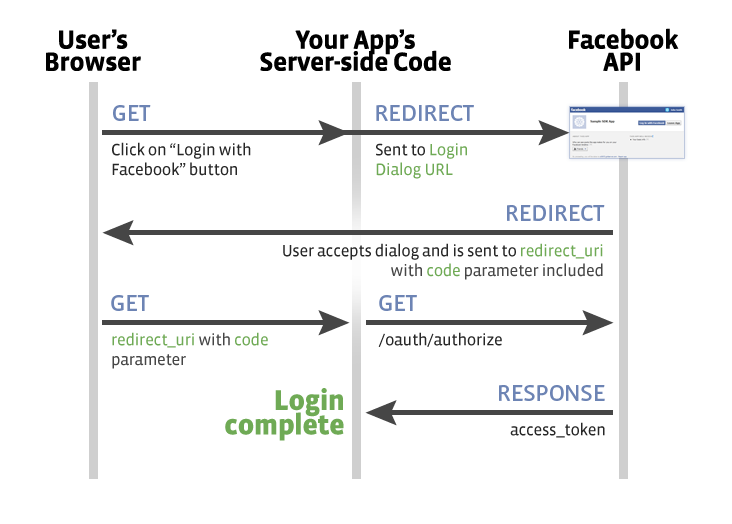
\includegraphics[width=5in]{figures/server-side-diagram.png}
\caption{Schéma přihlašování k facebooku pomocí OAuth}
(https://developers.facebook.com/docs/concepts/login/login-architecture/)
\label{fig:oAuthDiagram}
\end{center}
\end{figure}

Existují různé knihovny pro práci s facebook Graph API. Tyto knihovny se liší hlavně použitou platformou (Google Android, Apple iOS, ...) a programovacím jazkem (serverové: PHP, Java, apod., klientské: JavaScript). Některé z těchto knihoven mohou mít přihlašovací proces kvůli omezením mírně odlišný (například JavaScript), ale hlavní princip zůstává vždy stejný.

Nemusí se ale jednat pouze o aplikace pro interakci s facebookem, velké množství programů (například hry, kvízy a další) data z facebooku pouze čtou a získávájí informace o přátelích uživatele a podobně, které dále využívají ve hře. Takovéto aplikace jsou pak zobrazeny v okně facebooku (jsou vloženy do stránky pomocí HTML tagu iframe) a mohou používat facebookové prvky (tlačítka, vyskakovací okna, apod., všechna jsou popsána zde \verb|https://developers.facebook.com/docs/plugins/|), takže méně zkušení uživatelé si ani nemusí uvědomit, že používají aplikaci, která není vyvíjena facebookem. 

Facebook nepodporuje žádnou jinou možnost, jak aplikaci ovládat kromě Graph API. Kvůli častému zneužívání tohoto API byl ale facebook postupem času nucen některé funkce tohoto rozhraní omezit nebo úplně zakázat. Jedná se hlavně o možnost dát skupině nebo stránce na facebooku like anebo přidat si přátele. Tato funkce API byla ještě spolu s takzvaným likejackingem\footnote{Variace clickjacingu, pomocí HTML, CSS anebo JavaScriptu je na stránce skryto facebookové tlačítko like a je překryto jiným tlačíkem, uživatel pak po~kliknutí na viditelné tlačítko nevědomky aktivuje i skryté facebookové like tlačítko http://en.wikipedia.org/wiki/Clickjacking\#Likejacking} často zneužívána k podvodnému navyšování fanoušků facebookových skupin. 

\subsection{Omezení facebook Graph API}

Facebook proto zrušil možnost dávat stránkám like skrze Graph API. S~dalším zneužíváním funkcí facebook API se může stát, že budou dále zakázány i některé další funkce. Využití facebook API je tedy poněkud omezené a~s~nejistou budoucností. Hlavní nedostatky facebook Graph API pro využití pro experimentální aplikaci jsou:

\begin{itemize}
  \item nemožnost dát like skupině
  \item nemožnost přidat si nové přátele
  \item omezený výpis informací o osobě oproti webovému rozhraní
  \item časem mohou být zakázány nebo omezeny některé důležité funkce
\end{itemize}

Tyto nedostatky Graph API mi nedovolovaly jej použít pro implementaci  aplikace. Kvůli těmto omezením jsem si tedy vybral raději možnost obsluhovat facebook pomocí webového rozhraní za použití specializovaných programů a nástrojů k tomu určených.

\section{Možnosti ovládání webového rozhraní facebooku}

Po zamítnutí použití Graph API pro aplikaci jsem se zabýval dalšími možnostmi ovládání facebooku. Podrobněji jsem se zaměřil na jedno nízkoúrovňové a jedno pokročilejší řešení. První možností je využití protokolu HTTP. Druhou technologíí na kterou jsem se zaměřil byly programy pro simulování a ovládání webových prohlížečů.

\subsection{Výhody a nevýhody využití HTTP protokolu pro komunikaci s facebookem}

Jako první možnost ovládání webového rozhraní facebooku se nabízelo simulovat webový prohlížeč pomocí HTTP požadavků. Toto řešení je poměrně přímočaré a webový protokol HTTP je velmi dobře zdokumentovaný a jednoduše používatelný, později jsem ale tuto možnost zavrhnul, jelikož bych musel znovu implementovat již mnohokrát hotové řešení, kde bych musel řešit nízkoúrovňové problémy HTTP komunikace. 

Použití HTTP protokolu by se nejvíce vyplatilo u statických webových stránek. Největším problémem tohoto přístupu je ale skutečnost, že facebook používá velké množství AJAXových\footnote{AJAX - asynchronní načítání dynamických částí webových stránek pomocí JavaScriptu (viz http://en.wikipedia.org/wiki/Ajax\_(programming))} požadavků a dynamických JavaScriptových oken, které by mohly způsobit komplikace. 

Ztížilo by to především získávání informací z uživatelských profilů a podobně. Například pro zobrazení příspěvků na zdi uživatele za určité období, je potřeba dosáhnout konce stránky, kde se musí kliknout na tlačítko načíst další příspěvky a tento postup se opakuje, do té doby, než dosáhneme požadovaného množství nebo stáří příspěvků, stejný způsob zobrazování dalších dat se na facebooku používá i na dalších stránkách.

Mezi další nevýhody používání HTTP komunikace patří to, že facebook pro některé části webových stránek generuje odlišný HTML kód (mění se například atributy \verb|id| u HTML značek a podobně). Některé formulářové prvky pak mají jiné názvy a musel by se při každém požadavku zpracovávat HTML kód s formulářovými elementy. 

Nejvíce jsem se s těmito změnami setkal na hlavní stránce facebooku, kde pravděpodobně probíhá takzvané A/B\footnote{http://en.wikipedia.org/wiki/A/B\_testing} uživatelské testování stránek. To znamená, že se uživatelům zobrazují různé grafické verze stránky a následně se měří rozdíly úspěšnosti konverzního poměru měřených veličin (například: počet zobrazení stránky / počet nákupů) pro jednotlivé verze.

V poslední době se začal rozšiřovat nový internetový protokol nazvaný SPDY\footnote{http://en.wikipedia.org/wiki/SPDY}, který slouží jako nadstavba nad tradičním HTTP protokolem pro rychlejší načítání internetových stránek. Facebook tento protokol již na svých serverech používá a mohly by tak vzniknout problémy při HTTP komunikaci i když by měl být protokol SPDY teoreticky zpětně kompatibilní, nemuselo by vše být úplně bez problémů.

Kvůli těmto problémům spojeným s používáním HTTP protokolu jsem se tedy rozhodnul využít raději některé z hotových řešení a zabývat se komunikací s webovými stránkami facebooku na vyšší úrovni. 

\subsection{Programy simulující chování webového prohlížeče}

Jako nejjednodušší z možností ovládání webového rozhraní facebookové stránky se naskytlo využití programů, které simulují internetový prohlížeč. Existuje celá škála takovýchto programů. Téměř pro každý programovací jazyk existuje některý program, který dokáže zpracovávat webové stránky. Rozdíl mezi těmito programy je především v počtu a kvalitě implementovaných webových specifikací a funkcionalit.

Programy pro zobrazování webových stránek se liší především implementovaným vykreslovacím jádrem webového prohlížeče. V následujícím seznamu je zobrazen přehled nejpoužívanějších jader pro vykreslování webových stránek.

\begin{itemize}
  \item WebKit\footnote{Webkit - http://www.webkit.org/} - Apple Safari
  \item Blink\footnote{Spolčnost Google starající se o prohlížeč Chrome v~nedávné době oznámila, že již nadále nebude používat opensource jádro WebKit, ale vytvoří vlastní fork tohoto jádra s názvem Blink -  http://en.wikipedia.org/wiki/Blink\_(layout\_engine)} - Google Chrome
  \item Gecko\footnote{Gecko - https://developer.mozilla.org/en-US/docs/Mozilla/Gecko} - Mozilla Firefox
  \item Trident\footnote{Trident - http://en.wikipedia.org/wiki/Trident\_(layout\_engine)} - Microsoft Internet Explorer
\end{itemize}
 
Kromě těchto nejpoužívanějších vykreslovacích jader, které vyžívají nejznámější internetové prohlížeče, existuje i velké množství méně známých jader a v podstatě každý si může implementovat vlastní vykreslovací jádro pro webové stránky.

Vykreslovací jádro ovlivňuje to, jak bude webová stránka vypadat a jak bude interagovat. Každé webové jádro má své specifické chování a způsob vykreslování internetových stránek. Mohou se lišit způsoby vykreslení stejné webové stránky mezi jednotlivými verzemi stejného jádra. Existují i speciálně upravená jádra pro vykreslování internetových stránek na mobilních přístrojích, které často naschvál neimplementují některé pokročilejší funkce kvůli hardwarovým nárokům mobilních zařízení a rychlosti vykreslování celé stránky.

Druhým důležitým parametrem programů pro práci s webovým rozhraním internetových stánek je to, zda se webové stránky sestavují jen v paměti počítače, nebo zda se výsledek vykresluje i na obrazovku. Existují programy, určené především pro testování webových stránek, které pouze kontrolují výskyt a pozici jednotlivých elementů, ale nedokáží stránku vykreslit, mají vše uloženo pouze v paměti. Díky tomu jsou ale i rychlejší a jsou i implementačně jednodušší. 

Různé programy pro zpracování webových stránek jsou zobrazeny v tabulce \ref{tab:web-engines}. Jedním z nejpoužívanějších programů je pravděpodobně Selenium. Používá se především pro automatické testování webových stránek a~zdrojový kód je napsán v programovacím jazyce Java. 

\begin{table}[h]
\centering
\caption{Příklady programů pro zpracování webových stránek}\label{tab:web-engines}
\begin{tabular}{| l | c | p{5cm} | c |}
	\hline
	\textbf{Název} & 
	\textbf{Jádro} & 
	\textbf{Programovací jazyk/API} & 
	\textbf{Zpracování} \\ \hline
	
	Selenium & %\footnote{http://seleniumhq.org/} & 
	Gecko & 
	Java, C\#, Ruby, Python, PHP, Perl, Haskell, REST API & 
	vykreslení \\ \hline
	
	PhantomJs & %\footnote{http://phantomjs.org/} & 
	WebKit & 
	JavaScript & 
	paměť \\ \hline
	
	WebInject & %http://www.webinject.org/
	vlastní &
	XML API &
	paměť \\ \hline
	
	HtmlUnit & %http://htmlunit.sourceforge.net/
	vlastní &
	Java &
	paměť \\ \hline
\end{tabular}
\end{table}


Dalším používaným programem je PhantomJs. Jak už název napovídá, je tento program napsán v jazyce JavaScript. Hojně se používá pro vykreslování dynamických částí webového rozhraní internetových stránek přímo na serveru. Je to užitečné především pokud chceme poslat webové stránky pro vyhledávací roboty, kteří mají problémy se zpracováním JavaScriptu. 

Další programy uvedené v tabulce slouží především pro testování výstupu webových stránek a liší se především programovacím jazykem pro který je program určený a rozhraním pro práci s programem.

\section{Detailní popis programu Selenium}

Pro potřeby experimentu jsem se více zabýval programem Selenium, jelikož se jedná o nejvyzrálejší technologii s nejvíce možnostmi z dostupných programů. Původně program Selenium vznikl jako nadstavba webového prohlížeče Mozilla Firefox. Pomocí nainstalovaného pluginu v tomto prohlížeci jej lze ovládat přes programové API, které poskytuje program Selenium. 

Jedná se o Javový \verb|.jar| soubor, který se stará o spouštění a ovládání webového prohlížeče. API programu Selenium je nezávislé na programovacím jazyku a tak mohly vzniknout knihovny pro velké množství těchto jazyků. Selenium používá webové RESTové API, takže se dají na internetu najít i~neoficiální knihovny pro různé další jazyky, které nejsou podporovány přímo od výrobce tohoto programu. Dnes již existují k programu Selenium i pluginy, které umožňují místo prohlížeče Mozilla Firefox používat prohlížeče Google Chrome, Opera, PhantomJS a další.

Hlavní výhoda programu Selenium spočívá v tom, že jsou webové stránky renderovány ve skutečném internetovém prohlížeči a operace, které se v prohlížeči odehrávají vidíme v~reálném čase. V případě potřeby je možné převzít ruční kontrolu nad stránkou a pokračovat v interakci s webovou stránkou manuálně. 

S použitím reálného prohlížeče se pojí i výhoda optimalizace webových stránek facebooku. Stránky jsou pro reálný prohlížeč připravovány a zcela jistě jsou v něm facebookem důkladně testovány pro správné 
zobrazování a fungování všech částí. V případě nefunkčnosti by facebook všechny nedostatky co nejdříve napravil a určitě by velmi rychle reagoval na nahlášené problémy. (Facebook o některých nahlášených problémech ví, ale kvůli tomu, že pro něj nejsou natolik důležité se s nimi nezabývá, například nefunkčnost URL pro přidání podmínek pro používaní facebookové aplikace  nahlášena v prosinci 2012 - https://developers.facebook.com/bugs/393455200735878  není v dubnu 2013 opravena.) 

Selenium je produkt, pod kterým se skrývá soubor několika programů, které slouží primárně k testování internetových stránek přímo v prohlížeči. Původně se jednalo jen o rozšíření (takzvaný plugin) do prohlížeče Mozilla Firefox. Pomocí tohoto pluginu je možné nahrát konkrétní uživatelské chování na webové stránce (například: zadat konkrétní text do uživatelského pole, kliknout na tlačíto, otevřít novou stránku a podobně). Všechy akce se nahrávají a ukládají do souboru (s příponou \verb|.html|) a lze je jednoduše znovu opakovaně spouštět. Celý postup je totožný s používáním funkce makro pro~hromadné operace v programech jako jsou Microsoft Word anebo Adobe Photoshop. Tento program se nyní nazývá Selenium~IDE\footnote{http://docs.seleniumhq.org/projects/ide/}.

Díky oblibě tohoto pluginu se postupem času utvořil kolem této technologie celý ekosystém pro automatizované testování pomocí webového prohlížeče. Do tohoto ekosystému patří následující programy:

\begin{itemize}
  \item \textbf{Selenium IDE} - plugin popsaný výše
  \item \textbf{Selenium Remote Control} - program pro vyzdálené ovládání prohlížeče na jiných počítačích z různých programovacích jazyků
  \item \textbf{Selenium WebDriver} - program pro spouštění a  ovládání internetového prohlížeče lokálně
  \item \textbf{Selenium Grid} - za pomoci programu Selenium Remote Control dokáže spouštět webové prohlížeče na více serverech zároveň - hodí se především na paralelní testování stránek v odlišných prohlížečích a na různých operačních systémech
\end{itemize}

Více informací o jednotlivých produktech lze nalézt na oficiálních stránkách jednotlivých programů: \verb|http://docs.seleniumhq.org/projects/|. 

\subsection{Popis fungování programu Selenium WebDriver}

Pro naši aplikaci se nejlépe hodí program Seleinum WebDriver. Jedná se o programátorské rozhraní k ovládání celého prohlížeče z různých jazyků. Můžeme tak pomocí běžného programovacího jazyka napsat program, který spustí prohlížeč, provede v něm určené úkoly a poté prohlížeč zavře. To vše bez potřeby jakékoli lidské interakce, takže tyto úkony mohou být opakovatelné a prováděné na různých počítačích.

Celý mechanismus funguje na jenoduchém principu. Selenium WebDriver je v podstatě jen jeden \verb|.jar| soubor\footnote{spustitelný program napsaný v programovacím jazyce Java}. Jedná se o lokální webový server, který naslouchá na určeném portu našeho počítače a vystavuje RESTové rozhraní k ovládání prohlížeče. Z našeho programu se pak můžeme připojit k webovému serveru Selenium WebDriveru a posíláme na něj požadované akce, které se mají v prohlížeči vykonat. 

Jelikož je webové rozhraní programu nezávislé na programovacím jazyku, existují knihovny pro mnoho jazyků a je jednoduché dopsat si i vlastní knihovnu pro jakýkoli jazyk. Program Selenium WebDriver můžeme ovládat i pomocí nástrojů pro práci s HTTP protokolem (například cURL, HTTPie, apod.). Celé rozhraní je detailně popsáno na stránkách projektu\footnote{https://code.google.com/p/selenium/wiki/JsonWireProtocol}.

Program Selenium WebDriver používá k ovládání prohlížeče takzvané drivery. V~tomto případě se jedná o programy, které dokáží ovládat samotný prohlížeč - otevřít jej, otevřít konkrétní URL (viz ukázka: \ref{lst:seleniumOpenUrl}) a pohybovat se po stránce. Pozor, neplést s ovladači u hardware, nazývají se také drivery, ale jedná se o něco zcela jiného. 

\begin{lstlisting}[caption={Příklad otevření URL v programu Selenium WebDriver pomocí cURL},label=lst:seleniumOpenUrl,belowcaptionskip=0.4cm]
# Pomoci tohoto prikazu vytvorime novou session 
# (otevreme prohlizec firefox)
curl -X POST http://localhost:4444/wd/hub/session \
-d "{desiredCapabilities: {browserName: 'firefox'}}"

# Z predchoziho prikazu jsme ziskali sessionId
# sessionId pouzijeme v prikazu pro otevreni stranky
# :sessionId je potreba nahradit vysledkem predchoziho
# dotazu
curl -X POST \
http://localhost:4444/wd/hub/session/:sessionId/url \
-d "{url: 'http://www.facebook.com'}" 
\end{lstlisting}

Původně dokázal Selenium WebDriver ovládat pouze prohlížeč Mozilla Firefox, ale postupem času vznikly drivery i pro ostatní prohlížeče. V této době již můžeme použít Selenium WebDriver k ovládání následujících prohlížečů: Mozilla Firefox, Google Chrome, Microsoft Internet Explorer, Apple Safari, Android browser (defaultní prohlížeč na mobilních telefonech s~operačním systémem Google Android), iPhone browser (defaultní prohlížeč na mobilních telefonech Apple iPhone) a dříve zmíněných programů PhantomJS i HtmlUnit. 

Mimo driverů pro webové prohlížeče existují pro program Selenium WebDriver i dva speciální drivery: EventFiringWebDriver (slouží k odchytávání JavaScriptových událostí, které v prohlížeči vzniknou, můžeme na ně pak v našem programu reagovat) a RemoteWebDriver (slouží ke vzdálenému ovládání prohlížečů na jiných počítačích). S těmito drivery máme možnost ovládat všechny hlavní internetové prohlížeče a to jak desktopové, tak i mobilní.

Vývojáři prohlížeče Opera vydali 12. února 2013 
článek \cite{web:operaMovesToWebkit} o tom, že plánují svůj prohlížeč do budoucna postavit nad jádrem WebKit, které používají prohlížeče Google Chrome a Apple Safari. Pár měsíců po tomto oznámení vydali vývojáři prohlížeče Google Chrome dne 3. dubna 2013 na svém webu článek \cite{web:chromiumBlink} o tom, že vytvoří vlastní vykreslovací jádro Blink\footnote{http://www.chromium.org/blink}. Bude se jednat o fork doposud používaného opensource jádra WebKit. Do~budoucna bude určitě zajímavé sledovat, jak se celá situace nakonec vyvine, nicméně funkčnost programu Selenium WebDriver by to nemělo omezit.

\section{Výhody a nevýhody použití programu Selenium WebDriver}

Selenium WebDriver je program sloužící k ovládání internetového prohlížeče pomocí velkého množství programovacích jazyků. Největší výhodou používání programu Selenium WebDriver pro zpracování webových stránek je, že se stará o všechnu práci spojenou s komunikací skrze HTTP protokol, vykreslováním i ovládáním webových stránek a zpracováním všech dynamických skriptů na stránce. 

Selenium WebDriver nám umožňuje přistupovat k výsledným vyrenderovaným elementům prohlížeče a to jak textově, tak i k HTML zdrojům jednotlivých elementů na stránce. Problém nastává při následném zpracování, protože data ze stránky nejsou vždy jednotná jako v případě použití Graph API. Musíme tedy získaná data následně zpracovávat a upravovat.

Máme tedy k dispozici naprosto stejná data, jako uživatel internetového prohlížeče. Nemusíme se zabývat nízkoúrovňovými záležitostmi spojenými s fungováním internetu. Dále můžeme použít různé vykreslovací programy a webové prohlížeče a to včetně programů určených pro mobilní zařízení. Tento nástroj se nejvíce používá k automatickému testování webových stránek v různých prohlížečích a v této oblasti je velmi rozšířen. Můžeme k němu tedy nalézt velké množství návodů, knihoven, doplňků a rad na internetu. 

\textbf{Výhody využití programu Selenium WebDriver}

\begin{itemize}
  \item hojně používaný program
  \item možnost změny vykreslovacího programu
  \item velké množství vykreslovacích programů k použití
  \item možnost ručního ovládání browseru
  \item velké množství návodů, zdrojů a rad na internetu
  \item RESTové rozhraní pro ovládání browseru
  \item velké množství programátorských knihoven pro práci s tímto programem
  \item možnost přistupovat přímo k HTML zdrojovým souborům jednotlivých elementů na stránce
\end{itemize}

\textbf{Nevýhody využití programu Selenium WebDriver}

\begin{itemize}
  \item neexistuje oficiální knihovna pro jazyk PHP 
  od tvůrců programu Selenium
  \item nutnost spouštět celý browser - paměťově i časově náročnější
  oproti použití samostatné knihovny
  \item nutnost dále zpracovávat získaná data z textu nebo z HTML zdrojů elementů stránky
\end{itemize}

Pro náš experiment se program Selenium WebDriver hodí, jelikož výhody převyšují jeho nevýhody. Některé silné stránky, jako použití reálného prohlížeče, jsou vykoupeny pomalejším zpracováním. Pro experiment ale bylo důležitější použití reálného browseru, jako v případě procházení facebooku běžnými uživateli.

Neexistující oficiální knihovna pro jazyk PHP nakonec takovou nevýhodou nepřdstavovalo, jelikož se mi podařilo najít jinou kvalitní knihonvu pro tento jazyk, viz dále.

Nutnost zpracovávat získaná data by byla nutná u všech postupů mimo použití Graph API. Tato nevýhoda ale byla nahrazena výhodou, a to tím že můžeme používat všechny funkce facebooku bez omezení, které Graph API přináší a v některých případech jsme se dostali i k datům na stránkách, která nejsou pomocí Graph API dostupná.



\section{Využití aplikace}

Facebook koncem března 2013 oznámil, že má více než miliardu  aktivních měsíčních uživatelů (to znamená, že se přihlásí minimálně jednou za měsíc) \cite{web:fbMonthlyActiveUsers}. Takováto masa uživatelů je obrovská a díky tomu se z facebooku stal velmi zajímavý maketingový a komunkační nástroj. Díky obrovské oblibě facebooku tedy vzniky i internetové stránky zabývající se nákupem a prodejem aktivity na facebooku.

\subsection{Nákup aktivity na facebooku}

Na internetu se dnes běžně objevují nabídky na nákup fanoušků do facebookových skupin (příklady viz tabulka \ref{tab:likesBuy}). Ve většině případů se jedná o falešné nebo ukradené facebookové účty. Některé stránky jdou ale ještě dále a nabízejí na internetu možnost koupit si na facebooku falešnou přítelkyni (\verb|http://www.girlfriendhire.com/|, \verb|http://namorofake.com.br/| a další). 

\begin{table}[h]
\centering
\caption{Příklady webových stránek sloužících pro nákup like do skupin na facebooku}\label{tab:likesBuy}
\begin{tabular}{| l | c | p{5cm} | c |}
	\hline
	\textbf{Stránka} & 
	\textbf{Cena} \\ \hline
	
	http://get-likes.com/facebook-likes-store/ &
	1000 fanoušků za 30\$ \\ \hline
	
	http://fblikesmart.com/ &
	1000 fanoušků za 50\$ \\ \hline
	
	http://officialfacebooklikes.com/ &
	1000 fanoušků za 80\$ \\ \hline
\end{tabular}
\end{table}

Možnosti jsou různé od nákupu statusů od imaginární přítelkyně na vaši zeď nebo s vaším označením až po přidání do vztahu na facebooku. Nabízí se otázka, kolik účtů, které služby nabízí, je pravých a jaká je záruka, že po~zaplacení požadované částky  účty nezmizí. Každopádně se jedná o~zajímavý typ výdělku pomocí facebooku.

Exparimentální aplikace by šla jednoduše využít k podobnýmc účelům výdělku. Stačilo by na facebooku založit několik účtů, které by se pomocí této aplikace chovaly jako ostatní běžné účty. Následně by se v aplikaci nastavilo, které zaplacené statusy se mají kdy publikovat. Pravděpodobně by se muselo v aplikaci zapracovat na případech, pokud někdo uvedenou osobu kontaktuje. Upozornění na všechny tyto události se ale posílají~na e-mailovou adresu zadanou při registraci, takže se o nich dozvíme i tak.

\subsection{Ovádání osobních facebookových účtů}

Aplikace by šla jednoduše využít i na ovládání osobních facebookových účtů. Facebook nyní neumožňuje publikovat příspěvky v určitý čas, ale publikuje se vždy ihned po odeslání formuláře. Existují aplikace pro správu facebookových stránek sloužící především pro zjednodušení komunikace se~zákazníky, koordinaci publikování příspěvků na více facebookových stránkách a zobrazují statisky aktivity. Většinou jsou v takovýchto aplikacích zahrnuty i další sociální sítě jako jsou Twitter a podobně.

Všechny aplikace na správu facebookových stránek a účtú podle dostupných informací používají Graph API. Omezují se tedy pouze na dostupné akce, které toto API dovoluje používat. S využitím programu Selenium WebDriver můžeme ale využívat veškeré možnosti, které facebook nabízí.

Jednalo by se určitě o zajímavou možnost ovládání facebooku, například možnost naplánovat publikování příspěvku na určitý den a čas nebo automatické odpovědi na přijaté facebookové zprávy, stejně jako u e-mailů. Existují případy, kdy byli lidé vykradeni, kvůli tomu, že byli delší dobu mimo domov a zloději si to odvodili z toho, že dotyční na facebook nepřidali od~té doby žádný příspěvek anebo publikovali fotky ze zahraničních destinací. Další možností by bylo automatické zasílání přání k narozeninám přátelům na facebooku.



\chapter{Implementace}

\section{Požadavky na aplikaci}

Aplikaci pro ovládání účtů jsem nazval \textbf{Facebook client}. Před samotným vývojem aplikace jsem se zaměřil především na zjištění, které hlavní funkce bude program obsahovat a na které části se mám zaměřit. Důležité funkce aplikace pro ovládání účtů na facebooku byly následující:

\begin{itemize}
  \item přidávání přátel
  \item přidávání statusů na vlastní zeď
  \item přidávání účtu ke skupinám
  \item účast na facebookových událostech
  \item pozvání přátel na události
  \item stahování dat ze zdi profilu
  \item stahování dat z profilů přátel
\end{itemize}

Všechny tyto funkce byly do aplikace úspěšně implementovány a sloužily k automatizaci ovládání facebookových účtů.


\section{Volba technologií pro aplikaci}

Pro implementaci jsem si vybral především nástroje, které mi pro daný úkol přišly nejvhodnější a se kterými mám dostatečné zkušnosti pro bezproblémovou implementaci.

\subsection{Volba programovacího jazyka}

Pro implementaci celé aplikace jsem si vybral programovací jazyk \textbf{PHP}\footnote{http://www.php.net/}. Jedná se o dynamicky typovaný programovací jazyk s veřejným zdrojovým kódem, který se používá především k vytváření webových stránek a internetových aplikací. Tento jazyk jsem si vybral především proto, že s ním mám osobně největší zkušenosti a přijde mi na menší aplikace ideální. 

Díky dynamickému typování lze v tomto jazyce vytvořit aplikace velmi rychle. Protože aplikace neobsahuje složitý model a hlavní funkcionalitou je převážně volání RESTových služeb a ukládání nebo vybírání dat z databáze, přišel mi tento jazyk jako nejlepší možnost pro implementaci programu tohoto typu.

Celá aplikace facebooku je také napsána v jazyce PHP (i když používají speciální kompilátor pro tento jazyk - HipHop for PHP\footnote{http://en.wikipedia.org/wiki/HipHop\_for\_PHP}). Kromě jiných programů facebook uvolnil k volnému používání na internetu knihovnu pro~používání programu Selenium WebDriver\footnote{https://github.com/facebook/php-webdriver} pro jazyk PHP. Tuto knihovnu v aplikaci také používám pro komunikaci se Selenium WebDriverem.

Při rozhodování, který programovací jazyk pro aplikaci zvolím, jsem uvažoval i o jazyku Java, který je na rozdíl od PHP staticky typovaný. Jeho hlavní výhodou oproti jazyku PHP pro tento projekt byla knihovna přímo od tvůrců programu Selenium. Naopak nevýhodou byla nutnost výsledný program před spuštěním vždy překompilovat a tedy i pomalejší vývoj celé aplikace. 

Výhody jazyka Java se projeví až u větších a rozsáhlejších aplikací s rozsáhlým datovým modelem a pro takto malou aplikaci by se tyto výhody vykoupené pomalejším vývojem pravděpodobně nevyplatily. Po nalezení  knihovny PHP Webdriver jsem usoudil, že umí většinu potřebných akcí pro ovládání facebooku a není potřeba používat knihovnu pro jazyk Java.

Mezi další nevýhody jazyka Java patří to, že pokud chceme nasadit aplikaci na server, je složitější sehnat hosting a je náročnější nastavit celou aplikaci. Programy v jazyce PHP je možné nasadit i na sdílený hosting s~dalšími běžícími aplikacemi a konfigurace je jen minimální. Selenium WebDriver může běžet i na jiném serveru, protože veškerá komunikace probíhá pomocí HTTP protokolu.

\subsection{Volba databáze}

Jako databázi pro ukládání dat jsem pro začátek zvolil \textbf{MySQL}. Jedná se o open source relační databázi, kterou aktuálně vlastní společnost Oracle (viz \verb|http://www.mysql.com/|). Tato databáze je nejčastěji používána ve spojení právě s programovacím jazykem PHP. Do této databáze jsou ukládány informace o založených účtech, se kterými pracuje stahovací program. Jedná se o přihlašovací údaje (e-mail a heslo) a další údaje určené k~identifikaci účtu (jméno na facebooku, uživatelské jmeno na facebooku a id na facebooku).

Původně jsem chtěl pro ukládání stažených dat použít také MySQL databázi, ale rozhodl jsem se jinak. Pro ukládání dat stažených z uživatelských profilů se používá NoSQL (nerelační) databáze \textbf{MongoDB}. MongoDB je dnes jedna z nejrozšířenějších nerelačních databází. Jedná se o~open source dokumentově orientovanou NoSQL databázi o kterou se stará společnost 10gen (\verb|http://www.mongodb.org/|). Jedna z největších předností této databáze je to, že do ní lze ukládat jakákoli nestrukturovaná data ve~formátu JSON (JavaScript Object Notation - \verb|http://www.json.org/|) a pak lze s těmito daty nadále manipulovat a provádět nad nimi agregační dotazy. 

Databáze MongoDB byla vybrána hlavně proto, že umí pracovat s jakýmikoli nestrukturovanými daty, to znamená, že cokoliv, co získáme z~facebooku můžeme přímo bez úpravy uložit. Takovéto chování se hodí především k ukládání příspěvků ze~zdi facebookových uživatelů a informací z~profilových stránek osob. Nemusíme se starat o to, že někteří uživatelé mají omezenou viditelnost svých přátel nebo skupin. Kvůli těmto důvodům jsem si tedy pro ukládání stahovaných dat vybral databázi MongoDB vhodnou pro tuto úlohu.

Facebook v roce 2010 vyvinul vlastní NoSQL databázi nazvanou Cassandra (\verb|http://en.wikipedia.org/wiki/Apache_Cassandra|), která  slouží k~vyhledávání ve velkém objemu dat. Facebook tuto databázi později nahradil další nerelační databází  s otevřeným zdrohovým kódem nazvanou HBase (\verb|http://hbase.apache.org/|). Tyto databáze jsou ale určeny především k vyhledávání a jejich výhoda se ukáže až při ukládání mnohem většího množství dat, než bylo pro tento experiment potřeba.

\subsection{Volba webového frameworku}

Jako programovací jazyk bylo pro celou aplikaci zvoleno PHP, jak bylo zmíněno již výše. Pro tento programovací jazyk existuje kvalitní webový framework. Jmenuje se \textbf{Nette Framework} (\verb|http://nette.org/|) a hodí se především na menší aplikace. Jedná se o MVP (Model - View - Presenter) framework z dílny českého autora. Tento framework se stará především o zpracování webových formulářů, obsluhu požadavků webového prohlížeče, vykreslování HTML šablon a celkovou architekturu celé aplikace. Více informací o tomto frameworku je k dispozici v oficiální dokumentaci (\verb|http://doc.nette.org/|). 

Pro webové aplikace, které jsou rozsahem podobně velké jako je naše experimentální aplikace je tento framework ideální. Na internetu se dá najít velké množství návodů k tomuto frameworku v českém jazyce a existuje i početná česká komunita, která se tímto frameworkem zabývá a pomáhá s~vývojem. 


\section{Architektura celé aplikace}

Díky použití frameworku nette byla celá aplikace rozdělena podle paradigmatu MVP, tedy Model - View - Presenter. V~aplikaci jsou samostatně nahraditelné části pro práci s daty = model, šablony pro zobrazování dat = view a část, která se stará o zpracování uživatelských požadavků a propojení Modelu a View = presenter. Architektura celé aplikace se řídí doporučeními a zvyklostmi frameworku, například pro propojování tříd pomocí vkládání závislostí (takzvané dependency injection).

V aplikaci existuje pro každou sekci v navigaci samostatný presenter. Každý presenter se stará o vykreslování stránek  a zpracování formulářů pro~dané sekce. Dále aplikace obsahuje několik presenterů pro sprváný chod aplikace, například presenter pro zpracování chyb a podobně.

Model naší aplikace sestává ze samostatných servis (Service). Jedná se o~oddělené části aplikace starající se o konkrétní části modelu. Důležité jsou servisy pro uživatele (UserService), pro skupin (GroupService) a pro úkoly (TaskService). Tyto části aplikace se starají o zpracování odeslaných formulářů a ukládání dat do databáze. Poté jsou v aplikaci dvě servisy sloužící pouze k získávání dat z ostatních stránek. Jedná se o QuoteService a~InstagramService. 

Nakonec existují ještě dvě speciální servisy, jde o MongoService, která se stará o ukládání a vybírání dat z databáze MongoDB. Poslední a nejrozsáhlejší servisa se nazývá WebDriverService, stará se o ovládání programu WebDriver pomocí knihovny PHP Webdriver a o stahování a zpracování dat z facebooku. Pro zpracování dat získaných z facebooku slouží třída FbParser.

Vztah mezi třídami modelu a presenteru jsou vidět na obrázku \ref{fig:fcModelPresenter}.

View jsou vyřešeny tak, že pro každý presenter existuje samostatná složka se šablonami. Každá samostatná stránka má svůj soubor se šablonou a jménem odpovídajícím názvu stránky v URL. Pro celkové rozložení stránek existuje speciální šablona s názvem \verb|@layout|. Tato struktura je dána frameworkem Nette a pro zápis šablon se používá nástroj latte, který je součástí tohoto frameworku. 

\begin{figure}[h]
\begin{center}
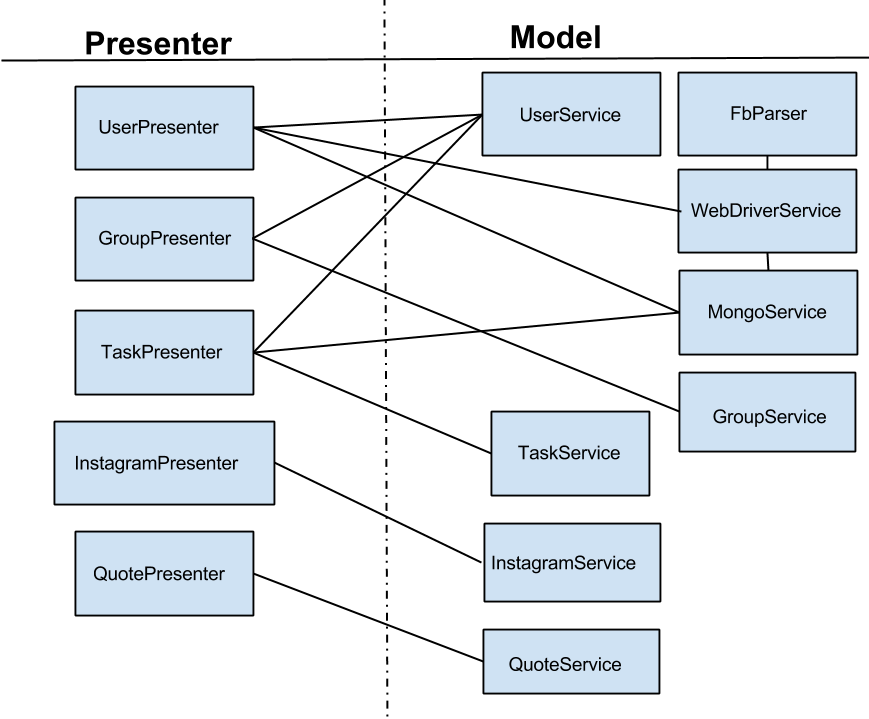
\includegraphics[width=5in]{figures/fcModelPresenter.png}
\caption{Přehled vztahů mezi třídami presenteru a modelu}
\label{fig:fcModelPresenter}
\end{center}
\end{figure}

\section{Rozdělení aplikace}

Aplikace sloužící pro otestování celého experimentu má dvě základní funkce. První z nich je sbírání dat o uživatelích facebooku z jejich profilů a inforamcí na jejich účtech. Druhou funkcí je ovládní experimentálních účtů, to znamená, nahrávání dat na facebook a interakce s dalšími uživateli. Data uživatelů z facebooku slouží k~analýze a k~dalšímu porovnání.

\section{Stahování informací z facebookových profilů}

Důležitou součástí aplikace je získávání informací o~uživatelích z~jejich facebookových profilů. Jak již bylo zmíněno v předchozí kapitole, vybral jsem pro stahování program Seleinum WebDriver, který je spouštěn pomocí jazyka PHP. Sesbíraná data jsou ukládána do databáze MongoDB nad kterou lze jednoduše vykonávat dotazy pro získání jakýchkoli statistických dat.

O veškeré zpracování stránek facebooku se stará program Selenium WebDriver, pomocí kterého se v prohlížeči Mozilla Firefox načte konkrétní stránka (například zeď anebo přátelé určitého uživatele). Z této stránky se poté přečtou jednotlivé fragmenty (například příspěvek na zdi anebo jméno přítele na facebooku) a tato data jsou pak pomocí PHP zpracována, upravena a uložena do databáze MongoDB. O tuto část aplikace se stará především WebdriverService.

Pro každý náš facebookový účet uložený v aplikaci je spuštěna následující sekvence operací:

\begin{itemize}
  \item stažení příspěvků na vlastní zdi
  \item stažení všech přátel, kteří si náš účet přidali
  \item stažení posledních příspěvků každého uživatele, kterého má účet v~přátelích
\end{itemize}

\subsection{Zpracování stahovaných informací}

Všechny statusy (příspěvky na zdi uživatele), které jsou stahovány ze zdi jsou pročištěny od nedůležitých dat a upravovány do stejné podoby. Data, která jsou získávána z facebooku, jsou někdy zobrazena rozdílně. Například zobrazení like u statusů. Pro analýzu statusů potřebujeme ukládat pouze počet like, které status obdržel. Facebook bohužel ale někdy místo počtu like zobrazuje i jména lidí, kteří like udělili. Stává se tak v případě, že like udělil, někdo z lidí, které má účet v přátelích anebo pokud je u statusu pouze jeden like. O veškeré zpracování a úpravu stahovaných informací se stará třída FbParser.

Pro účely experimentu se ukládá ke statusu pouze počet like, což je pro nás nejdůležitější údaj ohledně like. V programu se o získání počtu like stará funkce, která sečte počet jmen a počet like u statusu a vrátí výsledný součet like. 

Podobná situace nastává u komentářů u facebookových statusů. Pokud status obsahuje dva až čtyři nebo méně komentářů, tak se komentáře zobrazí i s textem. (Počet plně zobrazených komentářů se různí a není dán pevně pro každý status.) Pokud status obsahuje  více komentářů, tak se zobrazí text pouze dvou (až čtyř) posledních příspěvků v komentářích u statusu a všechny předchozí komentáře jsou skryté a zobrazí se až po kliknutí na~odkaz pro zobrazení starších komentářů. Naštěstí facebook v textu tohoto odkazu zobrazuje počet předchozích komentářů. Takže pro získání počtu komentářů nemusíme odkaz rozklikávat. 

Text dlouhých komentářů se navíc na facebooku zkracuje, pokud je příliš dlouhý. Většinou se zobrazí pouze prvních pět řádků komentáře. Pro zobrazení celého textu je potřeba rozkliknout odkaz na konci zkráceného textu a zobrazí se pokračování textu komentáře. 

Pro komentáře u skupin na facebooku se používá odlišný typ zobrazení než u statusů a osobních profilů. U statusů lidí na facebooku se zobrazují komentáře chronologicky podle data vložení, jen v jedné úrovni bez zanoření a pokud chce někdo reagovat na předchozí komentář, musí označit jeho autora pomocí znaku @ a jména jeho profilu na facebooku. 

U facebookových skupin se komentáře zobrazují ve dvou úrovních s jedním zanořením, to znamená, že pokud chce někdo reagovat na určitý komentář, tak se nový příspěvek odsadí, ale pouze u první reakce a je vidět jistá hierarchie. Nadále se komentáře u příspěvků skupin neřadí podle data přidání, ale podle oblíbenosti a relevance (tento algoritmus není veřejný, ale většinou rozhoduje počet like u komentářů). Stejný způsob komentářů facebook zobrazuje i u svého doplňku Facebook Comments\footnote{https://developers.facebook.com/docs/reference/plugins/comments/}, který nabízí pro ostatní webové stránky na vložení jako plugin. 

\subsection{Stahovaná data z facebooku}

Pro účely experimentu byla u statusů ukládána následující data získaná z~facebooku za použití programu Selenium WebDriver:

\begin{itemize}
  \item myWall - zda byl status stažen ze zdi našeho experimentálního účtu nebo ze zdi někoho z přátel účtu
  \item user - jméno uživatele, který status přidal
  \item fromUser - ze kterého účtu byl status stažen  
  \item status - text statusu
  \item commentsCount - počet komentářů
  \item likesCount - počet like
  \item timestamp - čas vložení statusu
\end{itemize}

Dále byli ukládáni do databáze všichni přátelé profilu. Struktura těchto dat byla následující:

\begin{itemize}
  \item name - uživatelské jméno přítele na profilu
  \item url - URL adresa profilu
  \item friendsCount - počet všech přátel stahovaného účtu, pokud to bylo možné z profilu zjistit
  \item mutual - počet společných přátel stahovaného účtu, pokud to bylo možné z profilu zjistit
  \item fromUser - kterého uživatele je stahovaný účet přítelem
  \item downloaded - čas stažení informace
\end{itemize}

Poslední stahovanou kolekcí do databáze MongoDB byly profily jednotlivých přátel našich profilů. Jedná se o informace o osobě, které o sobě každý na facebooku může vyplnit. Ukládaná data do této databáze jsou následující:

\begin{itemize}
  \item user - uživatelské jméno profilu
  \item friend - zda se jedná o přímého přítele nebo ne
  \item friendsCount - počet všech přátel stahovaného účtu, pokud to bylo možné z profilu zjistit
  \item photosCount - počet všech fotek stahovaného účtu, pokud to bylo možné z profilu zjistit
  \item likesCount - počet všech like skupin stahovaného účtu, pokud to bylo možné z profilu zjistit
  \item eduwork - pole informací o vystudované škole a zaměstnání
  \item family - pole jmen rodinných příslušníků a rodinných vztahů k dané osobě
  \item relationship - informace o partnerském vztahu účtu
  \item yearly - důležité mezníky v životě uživatele seřazené podle data (narození apod.)
  \item Bio - popis na profilu
  \item Birthday - datum narození 
  \item Gender - pohlaví
  \item Interested In - o které pohlaví se dotyčný zajímá
  \item Hometown - rodné město
  \item Current City - město, ve kterém daný účet právě žije
  \item Languages - jazyky, kterými účet umí mluvit
  \item Relationship Status - zda je daný účet v partnerském vztahu
  \item Religious Views - náboženské vyznání
  \item Political Views - politické vyznání
  \item Anniversary - výročí
  \item Mobile Phones - telefonní čísla
  \item Address - adresa bydliště
  \item Neighborhood - čtvrť
  \item Email - e-mailová adresa
  \item Facebook - adresa facebookového profilu
  \item Quote - oblíbené citace
  \item Screen Name - kontakty na různé komunikační kanály (Skype, ICQ, Jabber a další)
  \item Website - odkaz na webové stránky
  \item downloaded - čas stažení profilu
\end{itemize}

Všechny údaje, které začínají velkým písmenkem jsou parsovány přímo z~facebookové stránky. Jména klíče se tedy shodují s názvy oddílů na facebookové stránce. Začínají tedy proto velkými písmeny. Pro databázi MongoDB není v rozdílné velikosti písmen ani s mezerami u klíčů vkládaných dat žádný problém.

Některé z těchto informací nemusí být na profilech dostupné. Záleží vždy na konkrétním uživateli facebooku, zda je ochoten o sobě tyto informace prozradit a zveřejnit. Jediná povinná informace, která se zadává již při registraci na facebooku je pohlaví, takže pohlaví se na stránce s osobními informacemi o uživateli zobrazí vždy. 

Počet zobrazených informací na této stránce se navíc může lišit pro uživatele, kteří mají profil v přátelích a pro uživatele, kteří jsou pro profil cizí. Každá sekce má své vlastní nastavení viditelnosti. Možnosti viditelnosti jsou: veřejné (viditelné pro všechny), přátelé (viditelné jen pro~přátele), jen já (není viditelné pro nikoho kromě uživatele samotného) a vlastní nastavení (lze nastavit kteří konkrétní uživatelé nebo skupiny uživatelů mohou údaj vidět a pro které uživatele nebo skupiny je údaj naopak neviditelný).

Nová verze facebookového vzhledu zavedla na stránce s osobními informacemi nové sekce jako jsou: Hudba, Filmy, Seriály, Knihy, Místa, Like, Skupiny, Fitness a Poznámky. Protože byla aplikace nastavena pro starší verzi facebookové timeline, nepřidával jsem do stahování tyto informace, jelikož některé účty měly ještě starou verzi timeline a získávané informace by tudíž byly nekonzistentní.



\section{Problémy při implementaci}

Při práci na aplikaci jsem postupně narazil na různé problémy a překážky. Facebook je velmi rozsáhlá aplikace a využívá obrovské množství serverů po celém světě, aby mohl obsloužit všechny požadavky od uživatelů. Při~správě takto rozsáhlé aplikace je potřeba řešit problémy se synchronizací serverů a postupným zaváděním změn do uživatelského rozhraní.

Facebook je celosvětovou sociální sítí a je tedy přeložen do velkého množství jazyků (včetně pirátské angličtiny a angličtiny s písmenky obrácenými vzhůru nohy). Facebook je primárně vyvíjen v anglickém jazyce a do ostatních jazyků je celá aplikace přeložena. Překlad do všech jazyků probíhá pomocí speciální facebookové aplikace s názvem Translations \footnote{https://www.facebook.com/?app=1\&sk=translations}, kam mohou své překlady zasílat všichni uživatelé facebooku. (Dříve bylo například poměně dlouhou dobu v českém překladu špatně přeloženo slovo neděle jako slunce - anglicky Sun = slunce a zkratka pro neděli.) Jazyk procházených stránek pomocí programu Selenium WebDriver byl tedy vždy nastaven na~anglický, aby nedocházelo k problémům s měnícími se překlady. 


\subsection{Problémy se stahovaným časem}

Další problém při stahování dat z facebooku nastal při získávání času statusů a komentářů. Pro uživatele zobrazuje facebook na svých stránkách časové údaje v~různých formátech. První možností je relativní časový úsek od vložení, například: about a minute ago (přibližně před minutou), X minutes ago (před X minutami), X hours ago (před X hodinami) a podobně. Takovéto údaje se zobrazují u komentářů vložených před méně než 24 hodinami. 

Dalším zobrazovaným časovým údajem bývá: Yesterday (včera), Monday (pondělí) a podobně. Jedná se o statusy a komentáře vložené před více než 24 hodinami a méně než týdnem. Poslední možností zobrazení časového údaje je přesné datum, které se zobrazuje ve formátu: 15 April (15 duben). Navíc se liší zobrazený čas u statusů a komentářů pod nimi. U starších komentářů se zobrazuje i čas vložení, například: 2 February at 16:45 (2. únor v 16.45), kdežto u statusů se zobrazuje čas jen v ojedinělých případech.

Nevýhodou tohoto zobrazení časových údajů je, že nejsou vůbec přesné a časový rozptyl je až 24 hodin. Zkoumal jsem proto zdrojový kód stránky, zda jsou ve stránce dostupné i další údaje týkající se času vložení statusů a komentářů. Zjistil jsem, že element obsahující čas vložení má atribut \verb|title| s~textovou časovou reprezentací a atribut \verb|data-utime| s takzvaným unixovým časem (počet sekund od 1. ledna 1970), příklad elementu je vidět ve výpisu \ref{lst:timeElement}. 

\begin{lstlisting}[caption={Příklad elementu obsahující čas},label=lst:timeElement,belowcaptionskip=0.4cm]
<abbr 
  title="Tuesday, 23 April 2013 at 22:47"
  data-utime="1366750038" 
  class="timestamp livetimestamp">
    10 minutes ago
</abbr>
\end{lstlisting}

Stejné elementy používá facebook pro zborazení času u statusů a komentářů. Zkoumal jsem vztah mezi těmito dvěma časovými údaji uvedenými u~elementu. Zjistil jsem, že tyto dva časové údaje nejsou stejné. Stáhnul jsem tedy z facebooku 70 elementů s časovými údaji, z toho bylo 30 komentářů a 40 statusů. Všechna data byla získána ze tří rozdílných uživatelských zdí na facebooku. 

Zjistil jsem, že u 28 elementů byly údaje v rámci tagu stejné, u jednoho elementu se čas lišil o 1 hodinu, u 34 elementů byly časové údaje rozdílné o~8~hodin a u~7~elementů se čas lišil o 9 hodin. Přehledně jsou všechna data shrnuta v grafu \ref{fig:timeDifference}.

\begin{figure}[h]
\begin{center}
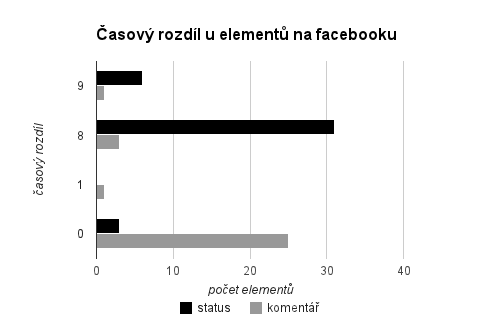
\includegraphics[width=5in]{figures/timeDifference.png}
\caption{Časový rozdíl u atributů title a data-utime u elementů zobrazujících čas na facebooku}
\label{fig:timeDifference}
\end{center}
\end{figure}

U některých elementů se dokonce lišil čas o rozdílný počet hodin u~statusu a odpovídajících komentářů pod ním. Tento problém bude pravděpodobně způsoben různými časovými pásmy. Facebook má několik datových center po  celém světě. Časový rozdíl 8 hodin odpovídá časovému posunu mezi západem USA a Greenwichským časem (základní časové pásmo). Rozdíl mezi Českou republikou a Greenwichským časem je pak 1 hodina. Různou kombinací těchto časových posunů pravděpodobně dojde k takovýmto rozdílům, které způsobují nekonzistence mezi časy uvedenými u stejného HTML elementu. 

Největším překvapením pro mne bylo to, že se různé rozdíly v časových údajích vyskytovaly na stejných zdech a dokonce se lišily i časové údaje u statusu a pod ním přidaných komentářů.  Je možné, že facebook vybíral statusy z jiných datových center než komentáře a tím vznikly tyto nekonzistence.

Nakonec jsem po tomto zjištění otestoval, který ze dvou stahovaných časových údajů odpovídá realitě. Test byl naštěstí poměrně jednoduchý. Vše jsem vyzkoušel vložením statusu a komentáře na facebook a poté jsem kontroloval, jak se obě data liší oproti realitě. 

Z tohoto testu jsem zjistil, že realitě odpovídá údaj vložený v atributu \verb|title|, tedy textová reprezentace data vložení. Pro data ukládáná do naší databáze jsem tedy používal tuto variantu pro parsování času.

Hlavní nevýhodou použití atributu \verb|title| pro parsování data je, že datum je uloženo ve formátu: Tuesday, 23 April 2013 at 22:47. Nemáme tedy k~dispozci údaj, ve které sekundě byl příspěvek vložen, ale pro náš experiment není tento údaj tolik důležitý. Pokud bychom potřebovali doplnit ve~které sekundě byl status nebo komentář vložen, mohli bychom tento údaj získat z druhého atributu elementu (\verb|data-utime|). 

\subsection{Změna webového rozhraní facebooku}

Největším problémem při použití programu Selenium WebDriver a vlastně jakéhokoli programu pracujícím s webovým rozhraním facebooku je fakt, že toto rozhraní se občas mění. Někdy se jedná o drobné změny, které běžní uživatelé této sítě ani nezpozorují. Jednou za čas na facebooku ale dojde k~razantnější změně webového rozhraní.

Během března 2013 facebook oznámil novou verzi profilové stránky (timeline) \cite{web:fbTimelineImprovements}. Jednalo se o jednu z větších úprav webového rozhraní facebooku. Tato nová funkčnost byla navíc spouštěna postupně, takže někteří facebookoví uživatelé mají starou verzi timeline a některé účty již používají verzi novou. Vše funguje tak, že pokud je na vašem profilu zapnutá nová verze timeline, tak vidíte novou verzi i na profilových stránkách všech vašich přátel. Ke staré verzi timeline se již po zapnutí facebookem nejde nikdy vrátit. Nelze ani ovlivnit, kdy bude nová verze zapnuta právě pro váš facebookový profil.

Pro čtení dat z facebooku pomocí programu Selenium WebDriver se používá XPath (XML Path Language). Což je jazyk pro vybírání elementů z XML a HTML dokumentů. Vše funguje tak, že se vybírají konkrétní elementy anebo se vybere jeden element a procházejí se jeho podelementy. Konkrétní elementy se vybírají podle atributů, především \verb|id| a \verb|class|, u~jednotlivých elementů.

Obával jsem se, že při změně vizuálního vzhledu timeline na facebooku budu muset předělávat velkou část stahování tak, aby aplikace mohla pracovat s novým HTML zdrojovým kódem. Naštěstí se ale HTML elementy na stránce měnily pouze minimálně. Takže stačilo upravit některé XPath dotazy a zbytek aplikace zůstal zcela funkční.

Změna timeline, která se částečně týkala i dalších stránek, ale měla jiný dopad. Na starém profilu se zobrazoval počet přátel, které má uživatel přidané na facebooku (pokud to neměl uživatel zakázané v nastavení). Se změnou na novou vizuální verzi timeline, ale tato položka zmizela a údaj o celkovém počtu přátel je dostupný až po přijetí žádosti o přátelství od~dotyčného člověka. V této chvíli tedy neexistuje žádný způsob, jak zjistit celkový počet přátel na facebooku u cizích profilů. Navíc byly skryty některé informace, které byly na staré verzi zobrazovány.

Facebook začal od dubna 2013 povolovat maximálně pouze 100 pozvaných uživatelů na událost najednou a každá událost může mít maximálně 300 nevyřízených pozvánek. Facebook tak nutí organizátory akcí vybírat jen hosty, které bude daná akce zajímat a budou se chtít účastnit \cite{web:fbEventsLimit} \cite{web:fbEventsLimitHelpCenter}.

Při programování aplikace bylo pozvání na události na facebook bez jakéhokli omezení. Pokud je nyní pozváno na událost na facebooku více než 100 osob, zobrazí se upozornění, že je potřeba pozvat pouze účty, které mají o danou akci skutečný zájem.


\section{Nahrávání dat na facebookové profily}

Druhá část aplikace pro experiment byla určena pro nahrávání dat na facebookové profily. Hlavním cílem pro přidávání dat na profily byla simulace chování reálných uživatelů a zvýšení věrohodnosti účtů.

\subsection{Možné způsoby interakce na facebooku}

Na facebooku je velké množství možností k interakci s ostatními uživateli. Nejdůležitějším prvkem na facebooku je zeď se statusy přátel. Statusy je možné komentovat, přidávat k nim like a sdílet (share = poslat na svou zeď pro zviditelnění svým přátelům). 

Kromě statusů lze na facebooku komunikovat pomocí zpráv. Systém je podobný jako u e-mailové pošty s tím rozdílem, že pomocí zpráv lze komunikovat pouze  v rámci facebooku. Zprávy jsou viditelné pouze pro uživatele přidané do komunikace, stejně jako je tomu u klasických e-mailových zpráv. 

Dalším komunikačním kanálem je chat, který probíhá v reálném čase. Facebookový chat je propojen se zprávami, takže veškeré informace, které jsou poslány přes chat, jsou viditelné i ve zprávách. Výhoda chatu oproti zprávám je, že  můžeme vidět, kteří uživatelé jsou právě online a zda si zaslanou zprávu již přečetli. 

Facebookový chat funguje pomocí otevřeného protokolu XMPP (Extensible Messaging and Presence Protocol). Tento protokol se používá pro komunikaci pomocí takzvaného Jabberu, takže pro používání facebookového chatu lze využít jakýkoli program podporující Jabber.

Další možností, jak na sebe na facebooku upozornit určitou osobu je možnost někoho šťouchnout (anglicky poke). Funkčnost tlačítka šťouchnout je jednoduchá. Pokud vás někdo šťouchne, přijde vám upozornění a můžete šťouchnutí opětovat.

\subsection{Implementované akce}

Při implementaci jsem se soustředil především na automatické nahrávání statusů na uživatelské profily. V implementované aplikaci je sekce Tasks (úkoly), kde je možné nastavit jaké akce se mají pro které profily provést. V aplikaci jsou implementovány následující automatické akce publikování na~facebook. Každá akce má jméno a parametry. Identifikátor je jednoznačné id na facebooku, které má každý prvek. Jedná se o několikamístné číslo a tento identifikátor lze získat z URL adresy na facebooku.

\begin{itemize}
  \item postStatus(text, [attachement]) - přidá na zeď uživatele status (parametr text), pokud je určena i příloha (attachement), což může být obrázek, video nebo odkaz, tak se vloží na facebook jako speciální objekt i s náhledem
  \item likeGroup(id) - přidat se ke skupině (Group nebo Page), parametrem je identifikátor skupiny 
  \item addFriend(id) - požádá konkrétního uživatele o přátelství na facebooku, parametrem je identifikátor uživatele
  \item rsvpEvent(id, [rsvpType]) - přidat se ke konkrétní události na facebooku, parametrem je identifikátor události, druhým parametrem je účast, možné hodnoty jsou: attend (účastnit se), maybe (možná), pokud není druhý parametr uveden, jako výchozí se bere možnost attend
  \item inviteEvent(id) - pozvat všechny facebookové přátele na událost, parametrem je identifikátor události
\end{itemize}

O ukládání těchto úkolů se stará v aplikaci TaskService a vše je ukládáno do databáze MongoDB. Ostatní typy možností komunikace na~facebooku nebyly automaticky zpracovávány. Nebylo by složité doimplementovat některé další funkce jako šťouchnutí všech přátel, ale pro tento experiment jsem se chtěl zaměřit na tyto hlavní funkce. 

Filosofie nahrávání na jednotlivé profily je taková, že v sekci Tasks se uloží všechny akce s volitleným přiřazeným uživatelem. Poté se při přihlášení k jednotlivým facebookovým profilům spustí pro každý profil provedení uložených úkolů na facebooku. Z nabídky se vyberou všechny požadované akce s tím, že jsou upřednostněny akce s nastaveným publikováním pro~aktuální účet (akce se zobrazují nejdříve a jsou odděleny od dalších úkolů). Uživatelské rozhraní nahrávání úkolů na facebookový profil je na obrázku \ref{fig:fcUserTask}.

\begin{figure}[h]
\begin{center}
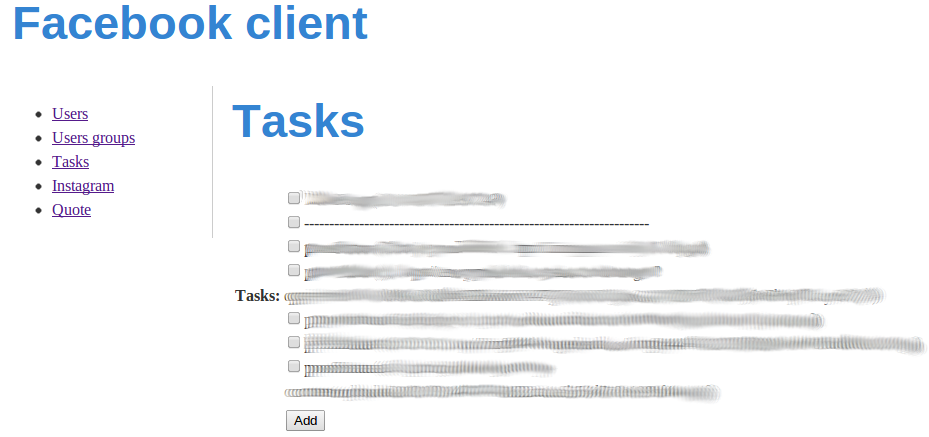
\includegraphics[width=5in]{figures/fcUserTask.png}
\caption{Uživatelské rozhraní nahrávání úkolů na facebookové profily}
\label{fig:fcUserTask}
\end{center}
\end{figure}

Celý datový model aplikace jsem shrnul na následujících přehledech. První přehled pro databázi MongoDB je na obrázku \ref{fig:mongoDataModel}. Druhý přehled se týká dat v databázi MySQL, ten je na obrázku \ref{fig:mysqlDataModel}.

\begin{figure}[h]
\begin{center}
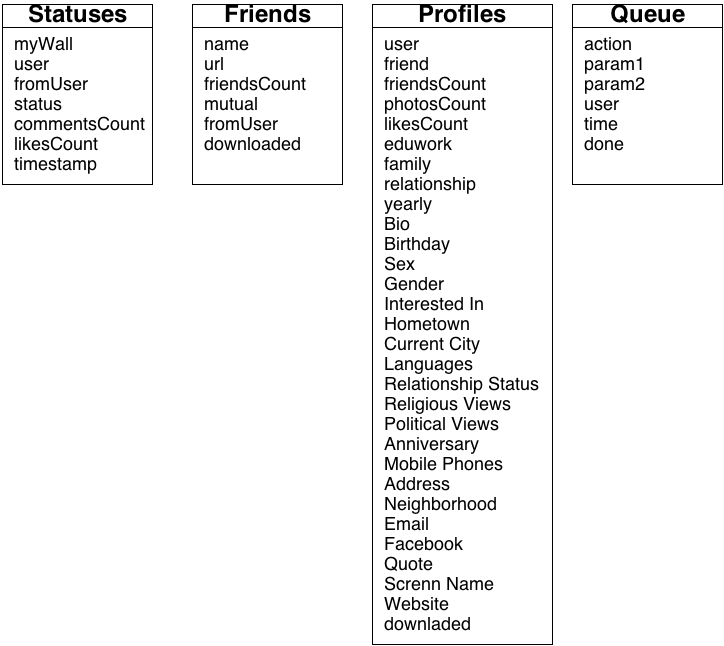
\includegraphics[width=5in]{figures/mongoDataModel.png}
\caption{Přehled ukládaných dat do jednotlivých kolekcí v databázi MongoDB}
\label{fig:mongoDataModel}
\end{center}
\end{figure}

\begin{figure}[h]
\begin{center}
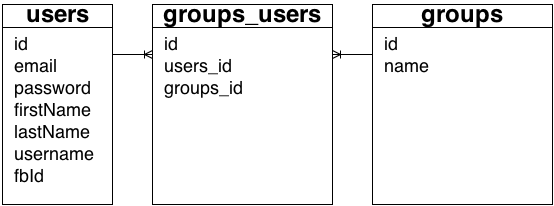
\includegraphics[width=5in]{figures/mysqlDataModel.png}
\caption{Přehled ukládaných dat do jednotlivých tabulek v databázi MySQL}
\label{fig:mysqlDataModel}
\end{center}
\end{figure}

\section{Části aplikace sloužící pro získání dat pro statusy}

Poslední části celé aplikace byly dvě pomocné sekce pro získávání dat z~jiných stránek. Jedná se o získání fotografií ze sociální sítě Instagram a získávání citátů z webové stránk citáty.net.

Instagram (\verb|https://instagram.com/|) je sociální sít, kam můžete nahrávat fotky z mobilního telefonu upravené pomocí různých filtrů. Jedná se tedy o obrovskou sbírku amatérských fotografií. Tuto sociální síť jsem vybral pro získávání obrázků nahrávaných jako statusy uložených účtů. 

Pro získávání fotek ze stránek instagramu jsem použil oficiální API na adrese \verb|http://instagram.com/developer/|. Vše funguje podobně jako Graph API pro facebook. Pro komunikaci s tímto API jsem na internetu vybral knihovou pro PHP \verb|https://github.com/galen/PHP-Instagram-API|. Přes toto API jsou pak z isntagramu vybírány fotky s určitým tagem, o vše se v aplikaci stará InstagramService.

Jak již název Quote = citáty napovídá, funkcí této části aplikace je získávání citátů pro nahrávání na facebookové profily. Jako zdroje vybíraných citátů jsem použil webové stránky \verb|http://citaty.net/|. Můžeme zde najít citáty slavných osobností, lidová pořekadla, přísloví a citáty, které nahrávají na stránky samotní uživatelé. 

Pro načítání citátů ze stránky \verb|http://citaty.net/| jsem použil knihovnu DOM (Document Object Model), která je součástí jazyka PHP. Vše funguje tak, že se pomocí PHP stáhne stránka s náhodým citátem, která má URL adresu \verb|http://citaty.net/nahodny-citat/|. Ze staženého textu se pak vybere pouze část s citátem, který se vypíše. O tuto funkčnost se v aplikaci stará třída QuoteService.


\section{Popis uživatelského rozhraní výsledné aplikace}

Uživatelské rozhraní výsledné aplikace je vidět na obrázku výpisu uložených facebookových účtů \ref{fig:fcUI}.

\begin{figure}[h]
\begin{center}
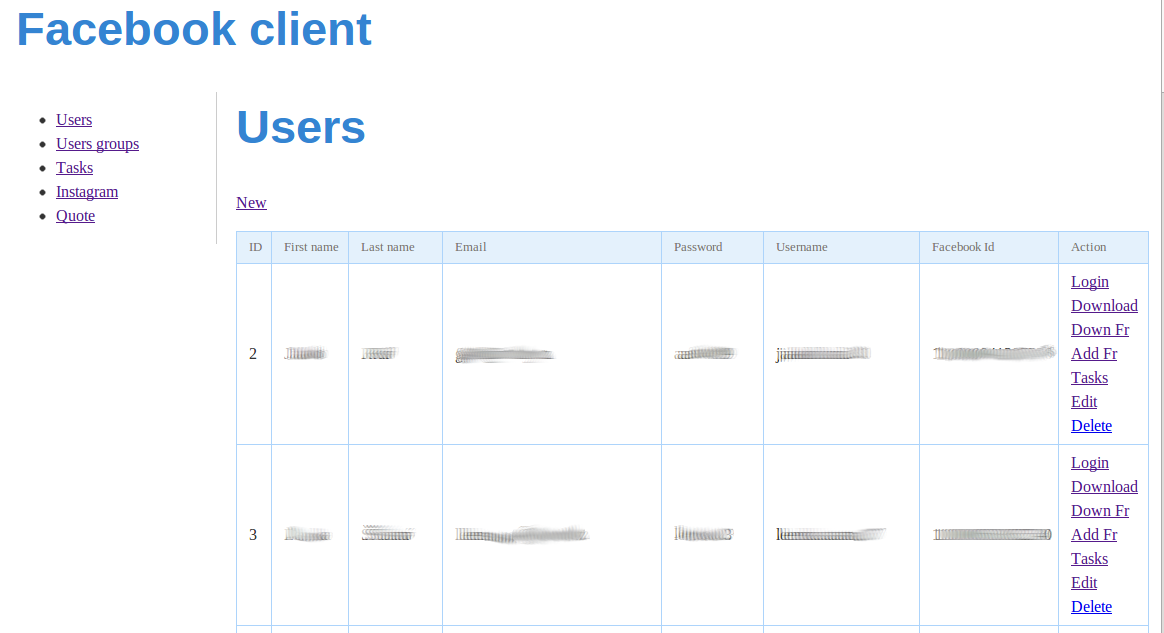
\includegraphics[width=5in]{figures/fcUI.png}
\caption{Uživatelské rozhraní výsledné aplikace}
\label{fig:fcUI}
\end{center}
\end{figure}

V levé části aplikace jsou sekce: Users (uživatelé), Users groups (skupiny uživatel), Tasks (úkoly), Instagram a Quotes (citáty). Každá z těchto sekcí má v aplikaci speciální část. Postupně stručně všechy tyto části popíšu.

Sekce users slouží pro uložení facebookových účtů které bude možné skrze aplikaci ovládát. U každého účtu máme uloženo jméno a příjmení, což slouží pouze pro jednodušší orientaci mezi účty, například při přidávání nových úkolů, ale stačilo by používat pouze e-mailovou adresu. Další uloženou informací jsou přihlašovací údaje, tedy e-mail a heslo k facebookovému účtu. Poslení dva údaje jsou facebookové uživatelské jmeno, zobrazené v URL adrese profilu, a facebookové číselné id profilu. Tyto údaje slouží pouze k identifikaci profilu při ukládání stahovaných informací do databáze. 

Pro každého uloženého uživatele v aplikaci můžeme provést následující akce. Akce Login slouží pouze k přihlášení daného uživatele, tato akce je důležitá, protože se uloží aktuální stav webového brosweru a další operace tak mohou pokračovat ve stejném okně. Download složí ke stažení dat z~uživatelské zdi, udělení like statusům na této zdi a stažení všech přátel daného účtu. Tato akce také zobrazí kolik je u účtu nových přátel, zpráv a~upozornění (notifikací) od posledního přihlášení.

Akce Download Fr (friends) se používá ke stažení informací na profilu, dat na zdi a přátel všech přátel daného účtu. Tato akce trvala delší dobu, takže nebyla spouštěna při každém přihlášení. Další možností, kterou lze pro každý účet pomocí aplikace dělat, je přidávání nových přátel, v aplikaci Add Fr (friends). Vše funguje tak, že se zobrazí vždy prvních 10 přátel, které facebook doporučí a pomocí zaškrtávacích polí se vybere, kterým účtům se má zaslat žádost o přátelství.

Nejdůležitější akcí pro každý profil je Tasks neboli úkoly, na této stránce lze vybírat uložené akce a provádět je na facebookových účtech. Přidávání úkolů bylo popsáno výše. Poslední dvě akce slouží k úpravě jakýchkoli informací  zobrazených na výpisu uživatelů (například pro změnu helsa), tato akce se jmenuje Edit a poslední akce Delete slouží k odstranění účtu.

Další část aplikace Users groups slouží k zařazování uložených profilů do skupin, například muži. Můžeme vytvořit neomezené množství takovýchto skupin a jednotlivé uložené účty lze k jednotlivým skupinám přiřazovat, jak je vidět na obázku \ref{fig:fcAssignGroup}. Skupiny slouží pro hromadné provádění akcí. Místo jednoho facebookového profilu lze vykonávané akce přiřazovat pro~celé skupiny.

\begin{figure}[h]
\begin{center}
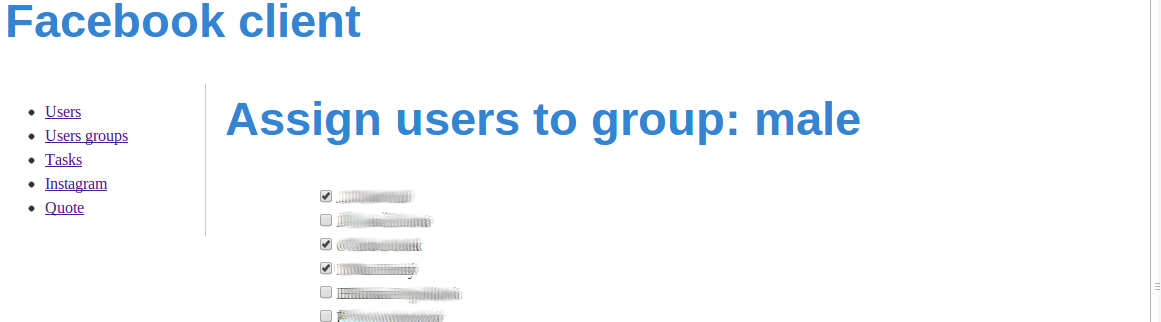
\includegraphics[width=5in]{figures/fcAssignGroup.png}
\caption{Přiřazování uložených uživatelů k jednotlivým skupinám}
\label{fig:fcAssignGroup}
\end{center}
\end{figure}

Důležitou částí aplikace byly úkoly, neboli Tasks. Zde se ukládaly veškeré akitvity, které bylo možné na uložených účtech vykonat. Celý proces funguje tak, že uživatel nejdříve uloží všechny akce. Například úkol přidat status, zadá text, volitelně i pro který účet nebo skupinu se má text zobrazit a vše uloží. Formulář pro přidávání nových úkolů je pro lepší pochopení celého procesu zobrazen na obrázku \ref{fig:fcNewTask}.

\begin{figure}[h]
\begin{center}
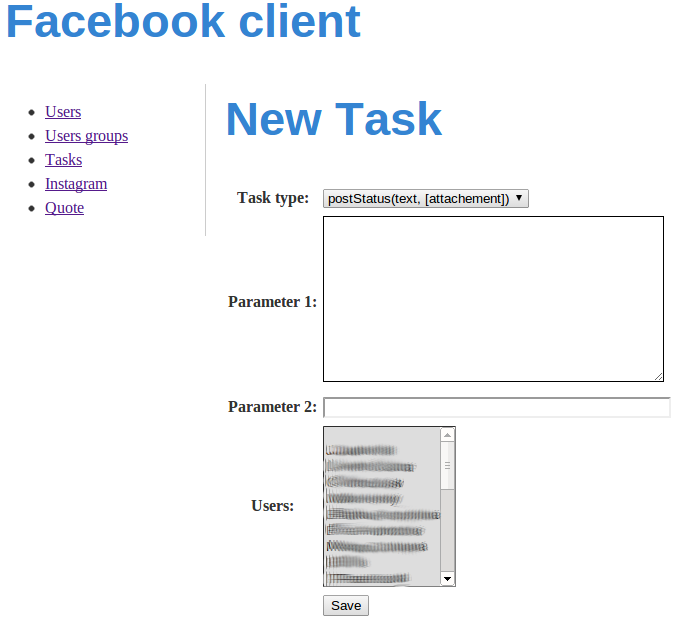
\includegraphics[width=5in]{figures/fcNewTask.png}
\caption{Formulář pro přidávání nových úkolů v aplikaci}
\label{fig:fcNewTask}
\end{center}
\end{figure}

Všechy uložené úkoly, které zatím nebyly použity lze vypsat. Na výpisu je u každého úkolu vidět identifikátor úkolu z databáze, typ úkolu, parametry, preferovaný uživatel (pokud byl nastaven) a čas uložení. Jakýkoliv úkol lze i smazat. Uživatelské rozhraní výpisu všech připravench úkolů je na~obrázku \ref{fig:fcTasks}. Po vykonání úkolu (sekce Users a akce taks) a provedení všech akcí na facebookovém účtu se úkolu nastaví příznak, že je již vykonán a ve~výpisu se již dále nezobrazuje.

\begin{figure}[h]
\begin{center}
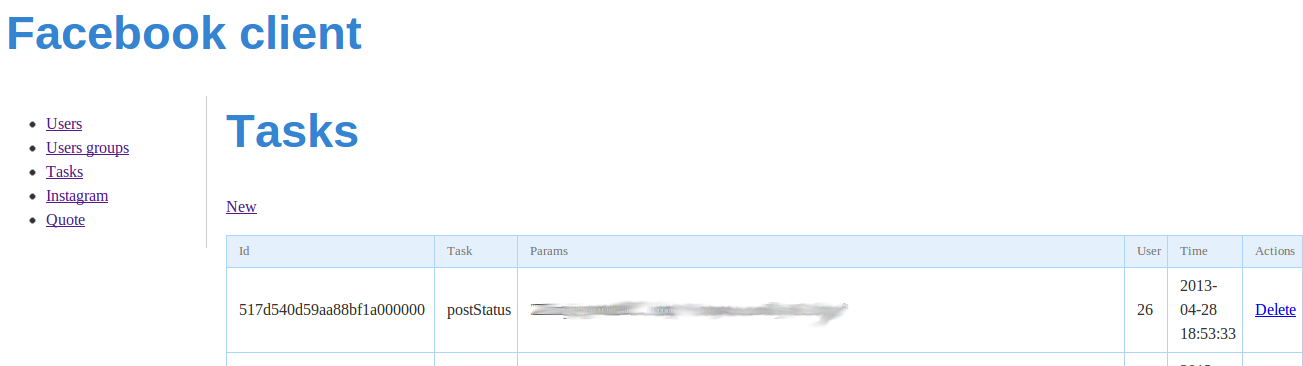
\includegraphics[width=5in]{figures/fcTasks.png}
\caption{Přehled připravených úkolů v uživatelském rozhraní aplikace}
\label{fig:fcTasks}
\end{center}
\end{figure}

Předposlední sekce se nazývá Instagram. Jedná se pouze o doplňkovou funkcionalitu aplikace. Tato sekce tedy sloužila k získávání náhodných obrázků. Vše funguje tak, že stačí zadat jakékoliv slovo (označení obrázk) a stránka vrátí obrázek včetně jeho URL adresy, která lze použít při nahrávání na~facebooku. Pokud se nám zobrazený obrázek nelíbí, pomocí tlačítka Refresh na stránce lze zobrazit jinou fotku.

Poslední sekce se velmi podobá té předchozí. Vybírají se vždy náhodné citáty ze stránek \verb|http://citaty.net|, kde je jejich obrovská sbírka. Aktualizací stránky se zobrazí citát další, jako v případě instagramu. Výhodou těchto dvou posledních sekcí je, že nemusíme opouštět naši aplikaci a máme vše potřebné k dispozici.



\section{Běh aplikace}

Celá aplikace byla spouštěna lokálně na mém počítači s operačním systémem Ubuntu Linux 12.04 LTS. Teoreticky by se dalo vše nahrát na~vzdálený server a ovládat přes internet, ale tím bychom ztratili výhodu kontroly prováděných operací v prohlížeči. Existují i internetové služby, které nabízejí pronájem výpočetního času ovládaných prohlížečů, takže lze mít celou aplikaci lokálně a spouštět program Selenium WebDriver přes internet vzdáleně. Problém je ale stejný jako v předchozím případě, nelze tyto prohlížeče ovládat a sledovat.

Pokud by se aplikace rozrostla anebo by ji používalo více uživatelů, pravděpodobně by se přenesení na vzdálený server vyplatilo. Přineslo by to ale problémy s nutností správy serveru a přísnějšího ošetřování neočekávaných stavů v aplikaci (například přidání formulářů do stránek, nebo neočekávaná vyskakovací okna).





\chapter{Průběh experimentu}

\section{Hlavní cíle experimentu}

Při přípravě celého experimentu jsem se chtěl zaměřit především na zjištění, kolik facebookových účtů bude ochotných přidat si neznámé facebookové uživatele. Dále jsem pak chtěl zjistit, kolik může získat fiktivní účet na facebooku přátel během jednoho měsíce. K tomuto účelu jsem připravil několik typů facebookových účtů a různé strategie možností přidávání prvních uživatelů facebooku.

Cílem těchto připravených strategií bylo zjistit, která bude nejúspěšnější z hlediska přidávání nových přátel. Dále pak na jakých faktorech záleží, zda se přidávají k účtu noví přátelé.

Dalším parametrem pro zkoumání bylo to, kolik založených účtů facebook během experimentu zablokuje a podle jakých kritérií. Zda je facebook schopný odhalit falešné účty a zda jak s nimi poté nakládá.

\section{Příprava experimentu}

Před samotným provedením experimentu jsem provedl některé akce nutné pro přípravu experimentu a otstovaní, jak by mohlo vše fungovat.

\subsection{První generace facebookových účtů}

Před samotným startem celého experimentu jsem potřeboval otestovat, jak přibližně bude vše fungovat a jak se budou účty pravděpodobně chovat. Založil jsem proto na facebooku pět testovacích účtů, které jsem nazval \textbf{první generace}. Pomocí těchto účtů jsem zjišťoval omezení i komplikace celého experimentu a jak by vše mělo fungovat. S využitím účtů z první generace jsem vyvíjel aplikaci pro automatické stahování a nahrávání dat na facebook (viz předchozí kapitola).

Pomocí první generace jsem ověřil, že facebook nekontroluje, pokud se z jedné IP adresy přihlašuje velké množství účtů. Denně jsem se přihlašoval k sedmi různým facebookovým účtům a nikdy jsem nenarazil na žádný problém. Je to i logické, jelikož v institucích jako jsou školy, knihovny a podobně se může k facebooku přihlašovat velké množství účtů, které jsou k internetu připojeny skrze jednu IP~adresu\footnote{IP adresa - číselná adresa počítače, pomocí které se připojuje k internetu}, přes kterou jsou tyto instituce připojovány k internetu.


\subsection{Zakládání e-mailových adres}

Před samotným provedením experimentu bylo potřeba založit facebookové účty pomocí kterých se bude celý experiment realizovat. Zakládání experimentálních účtů bylo poměrně složité, jelikož jsem chtěl původně spustit celý experiment v jeden den. Facebook při vytváření nového účtu kontroluje vždy IP~adresu počítače a nedovolí ze stejné IP adresy založit více než jeden účet denně. 

Pokud se někdo pokusí založit více než jeden účet, zobrazí se na facebooku obrazovka s nutností opsat kontrolní CAPTCHA\footnote{CAPTCHA - jedná se o ochranu internetových stránek proti robotům, nejčastěji je realizovaná nutností opisání textu z deformovaného obrázku} obrázek a po~úspěšném opsání facebook zobrazí stránku (viz obrázek \ref{fig:fbTelephoneNubmer}) s polem pro zadání telefonního čísla, na které má být zaslán aktivační kód. Nepokoušel jsem se pak už dále dostat přes tento krok, jelikož telefonní čísla se složitě shání a jedná se o osobní údaj, který jsem nechtěl facebooku sdělovat.

\begin{figure}[h]
\begin{center}
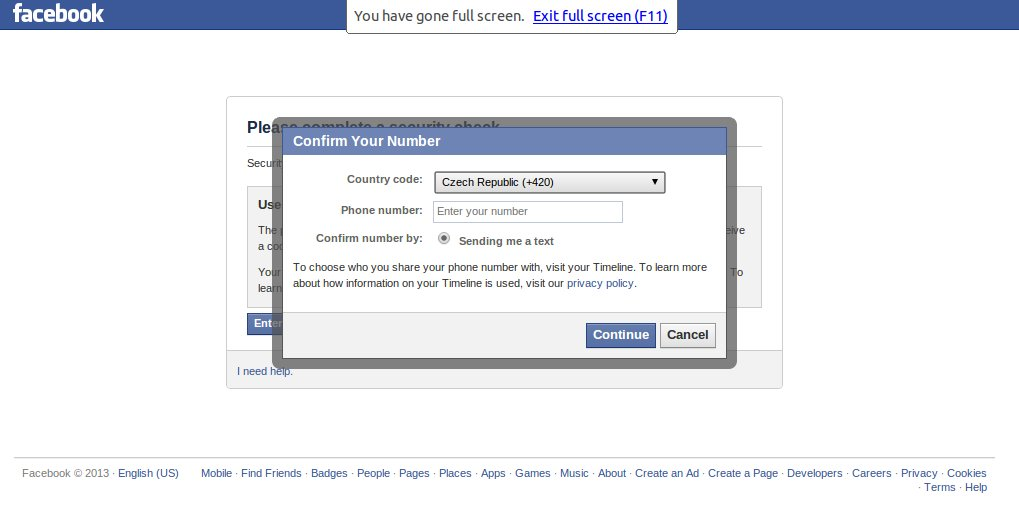
\includegraphics[width=5in]{figures/fb-telephone-number2.jpg}
\caption{Zadávání telefonního čísla pro ověření na facebooku}
\label{fig:fbTelephoneNubmer}
\end{center}
\end{figure}

Nejdříve bylo potřeba pro všechny facebookové účty založit e-mailové adresy, sloužící k vytvoření účtů na facebooku. Všechny e-mailové adresy byly založeny na české doméně s koncovkou \verb|.cz|, protože jsem chtěl provést experiment na uživatelích facebooku z České republiky a abych se mohl kvalitněji zaměřit na určitou skupinu uživatelů facebooku. 

Pro vytváření e-mailových adres jsem použil především bezplatnou e-mailovou službu od portálu \verb|http://www.seznam.cz/|. Jedná se v první řadě o internetový vyhledávač, e-mailové schránky jsou provozovány jako jedna z doplňkových služeb. Na tomto portálu lze vytvářet e-mailové adresy s~koncovkou \verb|@seznam.cz| a \verb|@email.cz|.

Pro každý experimentální účet na facebooku jsem nejdříve připravil náhodné jméno a příjmení. Hlavním požadavkem na jméno bylo, aby se jednalo o co nejvíce náhodné, ale zároveň i uvěřitelné jméno. Nechtěl jsem proto vytvářet nová jména, ale raději využít již existující. Ve velkém množství případů se jednalo o spojení různých křestních jmen a příjmení získaných ze~dříve stažených facebookových profilů (pomocí první generace). U~některých jmen bylo změněno i pohlaví příjmení. 

Nadále jsem pro vytváření jmen pro facebookové profily použil službu \verb|http://www.zlatestranky.cz/|. Jedná se o internetový seznam telefonních čísel fyzických a právnických osob v České republice. V současné době stránky obsahují pouze seznam právnických osob a změnila se grafika celých stránek, ale v době kdy jsem účty zakládal byl na stránkách i seznam fyzických osob. V dnešní době by bylo možné použít některý podobný internetový seznam fyzických osob.

Struktura e-mailových adres byla následující: \verb|jmenoprijmeni@domena.cz|. Přednost měla doména \verb|seznam.cz|, pokud byla e-mailová adresa s tímto jménem již zabraná, použil jsem doménu \verb|email.cz|. Pokud nebyla k dispozici ani tato e-mailová schránka, tak se za jméno vložila číslice (například: \verb|jannovak5@seznam.cz|) anebo byla použita modifikace křestního jména (domácký výraz, zdrobnělina a podobně).

Při vytváření e-mailových adres jsem na žádná omezení nenarazil. Webových stránek nabízejících bezplatně e-mailové adresy je velké množství a~to i pokud potřebujeme e-mailovou adresu pouze z české domény. Po~úspěšné registraci na facebook bylo vždy třeba aktivovat facebookový účet pomocí e-mailu. Facebook ihned po odeslání registračního formuláře zašle na e-mail zadávaný při registraci zprávu s ověřovacím odkazem. Aktivace účtu probíhá otevřením ověřovacího odkazu z e-mailu. Facebook tak kontroluje existenci a funkčnost této e-mailové schránky.

Facebook po úspěšné registraci na zadanou e-mailovou adresu posílá upozornění na různé aktivity, které se na facebooku dějí (například přijatá žádost o přátelství, obdržení facebookové zprávy, označení na fotce a podobně). Všechny možné typy zasílaných zpráv z facebooku lze upravit v uživatelském nastavení. Pro experiment byly e-mailové adresy důležité pouze k registraci facebookových účtu.

\subsection{Internetové služby poskytující dočasné a~veřejné e-mailové schránky}

Před začátkem experimentu jsem uvažoval nad použitím některé ze služeb poskytujících dočasné nebo veřejné e-mailové adresy. Jedná se o služby, které vám při návštěvě vygenerují náhodnou e-mailovou adresu (například:\newline \verb|e1461664@rmqkr.net|). Takovéto e-mailové adresy fungují většinou jen po~omezeně dlouhou dobu (v řádu několika desítek minut až hodin) a všechy e-mailové zprávy, které jsou odeslány na tuto adresu se zobrazí přímo na~navštívené stránce veřejně (u dočasných e-mailů jen pro návštěvníka, pro~kterého byla daná e-mailová adresa vygenerována).

Takovéto internetové služby slouží především jako ochrana proti e-mailové nevyžádané poště (takzvaný spam) a pro registraci na pochybné internetové služby. Po uplynutí časového intervalu bývá e-mailová adresa zrušena.

Příklady dočasných a veřejných e-mailových služeb:

\begin{itemize}
  \item \verb|http://10minutemail.com/| - vytvoří náhodnou e-mailovou adresu na různých doménách platnou 10 minut, tato doba lze postupně prodlužovat, vždy o dalších 10 minut
  \item \verb|http://mailinator.com/| - možnost zvolit si jakoukoli e-mailovou adresu na doméně \verb|mailinator.com| nebo \verb|spamherelots.com|, k této e-mailové schránce může přistupovat kdokoli, ale takováto e-mailová adresa má časově neomezenou platnost
  \item \verb|http://meltmail.com/| - funguje tak, že po omezenou časovou dobu přeposílá veškeré e-maily zaslané na vygenerovanou adresu na e-mail zadaný uživatelem, platnost vygenerovaných e-mailových adres může být 3, 6, 12 nebo 24 hodin
\end{itemize}

Zjistil jsem ale, že facebook registrace z takovýchto e-mailových adres blokuje a po registraci je ihned potřeba zadat telefonní číslo pro ověření totožnosti osoby, na které přijde ověřovací kód, stejně jako při registraci více účtů z jedné IP adresy. Dále se mi nepodařilo najít službu s dočasnými e-mailovými adresami, které by obsahovaly doménu s koncovkou \verb|.cz|. 

Použil jsem proto služby českých e-mailových serverů. Hlavní výhodou je to, že k e-mailovým schránkám jsem měl přístup i později a nebyl by pro~mne problém pokud by bylo potřeba dohledat některé informace posílané e-mailem (například zapomenuté heslo nebo důvod zablokování facebookového účtu).

\section{Problémy se zakládáním facebookových účtů}

Profily na facebooku tedy byly zakládány již dopředu, aby mohl být experiment spuštěn najednou ve stejný čas. Bohužel se ale stalo to, že dříve založené účty na facebooku byly neaktivní a když jsem se k nim přihlásil po delší době, tak facebook požadoval zadání telefonního čísla pro ověření totožnosti uživatele (stejně jako pokud se pokoušíme zaregistrovat více účtů denně z jedné IP adresy). Problém byl v tom, že facebook bere účty jako věrohodné až pokud mají přidáno několik přátel a vyvíjí aktivitu na facebooku. 

Stalo se tedy to, že jsem zakládal účty, aktivoval jsem je pomocí e-mailové adresy, ale už na účtech nebyla žádná další aktivita. Když jsem se poté v den spouštění experimentu k účtům vrátil, tak se mi objevilo textové pole s prosbou o ověření účtu zadáním telefonního čísla. Musel jsem tedy spustit experiment jen s funkčními účty s tím, že jsem po spuštění experimentu zakládal další nové účty.

Všechny facebookové účty jsem zakládal ručně, protože jsem se nechtěl v experimentu zabývat automatizací tohoto procesu. Celý experiment by šel rozšířit o tuto funkčnost, ale složitost tohoto problému je poměrně velká a v závěrečné kapitole popisuji, jak by šlo zakládání facebookových účtů teoreticky plně zautomatizovat.

\section{Skupiny facebookových účtů pro~experiment}

Při vymýšlení celého experimentu bylo hlavním cílem simulovat reálné chování uživatelů na facebooku. Chtěl jsem také vyzkoušet různé strategie přidávání přátel. Na začátku experimentu jsem tedy rozdělil všechny účty do pěti kategorií podle vyplněnosti profilu. Každá kateogie měla známku od 1 do 5, přičemž známka 1 znamená, že profil je nevyplněný a známka 5 znamená, že profil je zcela vyplněný. Hlavní motivací pro takovéto rozdělení je, že více vyplněné facebookové profily by měly být pro ostatní návštěvníky věrohodnější a lidé by si je měli teoreticky více přidávat.

Na následujícím seznamu jsou faktory ovlivňující \textbf{vyplněnost profilu}:

\begin{itemize}
  \item profilová fotka
  \item úvodní fotka (velká fotka na profilové stránce)
  \item vyplněny informace na stránce o sobě - především město ve kterém osoba právě žije, datum narození a oblíbené citáty
  \item veřejná viditelnost informací na profilu
\end{itemize}

Profily, které měly úroveň vyplněnosti na profilu 1, neměly použitou ani jednu z možností uvedených výše. Profily s úrovní 2 měly náhodně vybranou jednu z výše zmíněných možností pro zatraktivnění profilu. Profily s úrovní 5 měly vyplněny všechy výše zmíněné možnosti.

Na začátku experimentu jsem očekával, že profily s více vyplněnými daty na facebooku budou pro nové přátele atraktivnější a budou se s nimi chtít více přátelit. Důležité ale pro celý experiment bylo, jak velké budou rozdíly mezi těmito skupinami a jak moc bude tato metrika přidávání přátel ovlivňovat.

Pro získání fotografií k profilům posloužily veřejné internetové seznamky a sociální sítě. Z českého prostředí se jednalo především o webové stránky: \verb|http://libimseti.cz/| a \verb|http://www.lide.cz/|. Ze zahraničních webů posloužila nejlépe internetová stránka \verb|http://www.myspace.com/|. Výhodou těchto stránek je, že lze vybírat profily podle pohlaví a věku, což bylo ideální, protože bylo jednoduché najít profilové fotky odpovídající pohlaví a věku jakéhokoli experimentálního facebookového profilu. Veškeré obrázky jsou navíc veřejně dostupné bez nutnosti přihlášení na zmíněné služby.

Původně jsem chtěl do experimentu zahrnout i možnost zasílání stejných statusů na různé profily a zjišťování jak budou úspěšné. V aplikaci k tomu sloužily skupiny uživatelů. Při zjišťování reakcí uživatelů pomocí první generace jsem ale narazil na to, že aktivita (like, komentáře a sdílení) u statusů nebyla vůbec žádná. 

Každopádně v aplikaci zůstala možnost hromadného přidávání úkolů na každý facebookový účet v dané skupině. Ve výběru uživatelů při přidávání úkolů stačí místo konkrétního uživatele vybrat konkrétní skupinu.

\subsection{Strategie přidávání prvních přátel na~facebooku}

Pro vytvořené facebookové účty jsem pro experiment vytvořil pět různých strategií přidávání nových přátel. Cílem bylo otestovat, jak úspěšné strategie budou a zda bude rozdíl v počtu přidaných přátel mezi různými strategiemi. 

\textbf{Strategie přidávání} nových přátel:

\begin{itemize}
  \item \textbf{many friends} - přidávání osob s vysokým počtem přátel na facebooku
  \item \textbf{fake profiles} - přidávání falešných facebookových profilů
  \item \textbf{facebook suggestions} - přidávání profilů na facebooku, které doporučí facebook 
  \item \textbf{mutual friends} - přidávání profilů s největším počtem společných přátel
  \item \textbf{facebook groups} - přidávání skupin na facebooku a následné přidávání profilů, které mají u skupiny like
\end{itemize}

Všechny experimentální účty byly zařazeny do jedné z těchto pěti skupin. Toto rozdělení profilů bylo ještě navíc zkombinováno se skupinami vyplněnosti profilů popsaných výše. V každé skupině bylo tedy vždy pět účtů s~různou skupinou vyplněnosti. Vznikl tak soubor pětadvaceti facebookových profilů, z nichž každý byl zařazen do jiné skupiny vyplněnosti a také rozdílné skupiny pro přidávání nových přátel.

Před spuštěním experimentu jsem očekával, že nejúspěšnější budou strategie many friends a fake profiles. Profily s velkým množstvím uživatelů si podle předpokladů budou do svých přátel přidávat i neznámé facebookové profily. Majitelé účtů s velkým počtem přátel na facebooku jsou ve většině případů známé osobnosti nebo osoby pro něž je facebook reklamním nástrojem, například hlasatelé v rádiu, tvůrci vtipných videí a podobně. Pro tyto osoby je důležitý počet přátel a ve velké míře si přidávají účty, které nikdy v reálném světě nepotkaly. Tyto účty s vysokým počtem přátel jsou tedy zvyklé přidávat si nové přátele na facebooku.

U falešných profilů jsem předpokládal, že to bude podobné, jelikož jsou pro tyto účty nejdůležitější přátelé na facebooku. Předpokládal jsem tedy, že si budou neznámé účty také přidávat bez problému. Očekával jsem, že tyto dvě strategie budou pro nasbírání největšího počtu přátel na facebooku nejúspěšnější.

U některých profilů zařazených do určitých skupin přidávání nových přátel na facebooku bylo nutné ze začátku přidat první přátele. Jednalo se o skupiny many friends a mutual friends, tyto strategie používaly již existující přátele u profilu. U těchto skupin byly první uživatelé přidáni z~některé náhodně vybrané skupiny na facebooku. 

K přidávání prvních přátel jsem využil facebookové pluginy, které jsou veřejně dostupné na některých internetových stánkách. Jedná se o takzvaný facebook like box \cite{web:fbLikeBox}, kde jsou zobrazeny profilové fotky a odkazy na facebookové profily uživatelů, kteří mají danou stránku v oblíbených. Využil jsem tedy takto veřejně dostupné náhodné facebookové profily a přidával je k experimentálním účtům ve výše zmíněných skupinách.

V původním plánu bylo využití událostí a her na facebooku pro přidávání nových přátel, ale po vyzkoušení na první generaci jsem tento způsob zavrhl. Prvotní myšlenka byla taková, že se experimentální účet bude přidávat na~facebookové události a bude si postupně přidávat účastníky akcí. Po vyzkoušení jsem ale zjistil, že je k tomuto účelu lepší využít facebookové skupiny. Velké množství událostí s vysokým počtem účastníků zakládají kluby nebo organizace a ty mají ve většině případů založeny své facebookové skupiny, pomocí nichž akce promují. Navíc si uživatelé těžce spojovali souvislost mezi událostí a zaslanou žádostí o přátelství.

Využití facebookových her pro přidávání nových přátel by mohlo být velmi zajímavé, jelikož ve hrách existují různé výhody za~zaslání pozvánek facebookovým přátelům a někdy můžete přátele na facebooku požádat, aby vám poslali některé vylepšení nebo s nimi vyměňovat suroviny ve hrách. Čím více přátel na facebooku do hry tedy účet pozve, tím větší výhody ve~hře získává. Při hraní her bývá běžné, že si uživatelé zakládají na facebooku nové účty jen aby mohli získat co nejvíce těchto výhod.

Bohužel má ale každá hra jiné ovládání a velké množství her je napsáno v technologii Adobe Flash\footnote{Adobe Flash - http://www.adobe.com/products/flash.html} nebo podobných, které nejsou přístupné přes HTML zdrojový kód stránky a nešel by tedy pro interakci s nimi použít program Selenium WebDriver. Pro ovládání těchto her by musel být vyvinut mnohem složitější způsob procházení stránek. Musel jsem tedy od tohoto záměru upustit, ale jedná se o zajímavý segment, kde by se mohly účty sami doporučovat a posílat pozvánky na facebooku.

Je důležité zmínit, že žádné dva experimentální účty nebyly sobě navzájem přáteli na facebooku. V pozdější fázi se některé aktivní facebookové účty staly přáteli více experimentálních účtů, ale záměr byl co nejvíce simulovat chování reálných uživatelů a aby byly počáteční přátelé účtů co nejvíce náhodní.

Celkově jsem kvůli problémům se zakládáním facebookých účtů pracoval s 25 experimentálními účty. Z toho 14 účtů představovalo ženy a zbývajících 11 účtů bylo mužských. 

K~těmto účtům jsem se přihlašoval vždy jednou za čtyři dny. Vše vycházelo tak, že jsem se za den přihlásil k~osmi až devíti účtům z těchto pětadvaceti. Za jeden týden jsem se tedy ke~každému experimentálnímu účtu přihlásil přibližně dvakrát s tím, že pokud se u některého účtu objevilo podezření z jakékoli nestandardní činnosti. Provedl jsem požadované akce pro daný účet a pokračoval jsem s dalšími účty v sérii až následující den.

Po každém navštívení všech pětadvaceti účtů jsem provedl jednodenní pauzu a nepřihlásil jsem se k žádnému z experimentálních účtů. Navštívení všech účtů i s pauzou tedy trvalo celkem 4 dny. Přihlašování probíhalo v~pravidelných půltýdenních intervalech.

Začátek experimentu byl naplánován na začátek dubna 2013 a trval přesně 32 dní. Všechny účty byly za tuto dobu běhu experimentu navštíveny přesně devětkrát. Výsledky získané během toho experimentu byly velmi zajímavé.

\subsection{Fáze experimentu}

Strategie přidávání přátel popsané v předchozí kapitole byly využívány ze~začátku experimentu, když bylo potřeba nabrat určitou základnu přátel na~facebooku, aby profil vypadal pro ostatní facebookové uživatel jako aktivní a důvěryhodný. Tato fáze trvala dva a půl týdne a hlavním cílem bylo získat přátele, kteří budou ochotni přijmout žádost o přátelství na facebooku od~experimentálních účtů. 

V pozdější fázi experimentu byla využívána pouze strategie facebook suggestions. Tato strategie totiž počítala s přidanými přáteli k experimentálnímu účtu a pracovala hlavně se společnými a naposledy přidanými přáteli. Hlavní výhodou bylo, že se přidávali uživatelé z podobných okruhů a přátelé přátel. Ostatní strategie pouze přidávaly nové účty bez jakýchkoli vazeb na stávající facebookové přátele. 

Celý experiment probíhal tak, že jsem pro každý sledovaný účet nejdříve spustil stahování všech dat z profilu. V rámci tohoto stahování se stáhla zeď přihlášeného účtu a při té příležitosti byl udělen like třem statusům uživatelů (statusy od facebookových stránek se přeskakovaly) s~nejvyšším počtem like.

Pro přidávání like ke statusům se procházelo pouze dvacet prvních statusů na stránce, aby nedocházelo k přidávání like k neaktuálním statusům. Při menším počtu přátel u experimentálního účtu na facebooku se totiž zobrazovaly na zdi statusy starší než několik měsíců. Všechny parametry, tedy počet přidaných statusů za jedno příhlášení i počet statusů pro které se počítá počet like by šlo upravit, ale tyto hodnoty mi přišly při testování na první generaci ideální.

Občas se stávalo, že všechny tři like u statusů za jedno přihlášení získaly statusy jednoho uživatele na facebooku. Jednalo se především o velmi aktivní profily s velkým počtem přátel - tím pádem měly velký počet like u veškeré své aktivity na facbooku a zároveň se na zdi zobrazovalo velké množství jejich statusů. Vše by šlo vylepšit kontrolováním autorů statusů a přidáváním like pouze u jednoho statusu pro každého autora. Naštěstí k~přidávání like u statusů pouze jednoho uživatele nedocházelo často, takže jsem algoritmus neměnil.

Po stažení všech informací přišlo na řadu nahrávání informací na uživatelské profily. Pro každý profil bylo připraveno několik možných statusů na~nahrání na facebook a stačilo jen vybrat konkrétní status a odeslat formulář. Statusy je možné připravit dopředu a přiřadit pro přidání na konkrétní profil nebo pro kterýkoli profil.

Přidávání přátel na facebooku probíhalo podobným způsobem. Nejdříve se otevřelo okno pro přidávání přátel daného profilu. Na pozadí se stáhlo prvních 10 přátel, které facebook danému profilu doporučil. Jedná se o~stránku: \verb|https://www.facebook.com/find-friends/browser/|. Experimentální aplikace zobrazila jména těchto doporučených přátel a bylo možné vybrat, kterým uživatelům bude zaslána žádost o přátelství. 

Ze začátku jsem chtěl při experimentu vždy automaticky zaslat žádost o přátelství prvním pěti nabídnutým facebookovým účtům, ale při~testování na první generaci jsem zjistil, že se takto k profilu přidávaly účty ze~zahraničí, které nerozumněly přidávaným statusům. Chtěl jsem, aby nově přidávané profily byly převážně z České republiky, proto bylo potřeba přidat mezikrok s vybíráním relevantních přátel.

\subsection{Četnost přidávání přátel}

Hlavním cílem interakce na facebooku byla věrohodnost pro ostatní facebookové uživatele. Ze začátku jsem po zaregistrování nového profilu plánoval přidávat pokaždé přibližně osm přátel. Když se zaregistruje nový uživatel na facebook, tak nemá skoro žádné možnosti využití, dokud nemá nějaké přátele, většina uživatelů se tak snaží zpočátku přidávat více přátel. 

Facebook ihned po registraci nového profilu nabízí možnost stáhnutí kontkatů z e-mailu, z programu Skype nebo z programu ICQ za účelem nalezení nových přátel na facebooku. Vše funguje jednoduše tak, že stažené kontaktní údaje se porovnávají s registrovanými uživateli facebooku a pokud se najde shoda, tak facebook nabídne tyto účty ke vzájemnému spřátelení.

Facebook ale při přidávání některých přátel (nepdařilo se mi najít žádné zjevné spojitosti) zobrazil potvrzovací okno, viz obrázek \ref{fig:confirmFriendship}. Jedná se o~potvrzení, zda známe daný facebookový účet i v reálném světě. Tento dialog stačí potvrdit a vše funguje. Facebook tím do jisté míry kontroluje, aby si uživatelé přidávali pouze přátele, které znají.

\begin{figure}[h]
\begin{center}
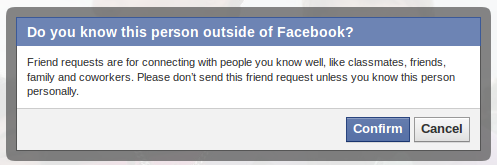
\includegraphics[width=5in]{figures/confirm-friendship.png}
\caption{Potvrzení zda se znají osoby v reálném světě při zasílání žádosti o~přátelství na facebooku}
\label{fig:confirmFriendship}
\end{center}
\end{figure}

U některých účtů, především s málo přidanými přáteli, se mi ale stávalo, že se zobrazilo podobné okno jako v předchozím případě. Jednalo se ale o~nepovolení zaslání žádosti o přátelství facebookem. Obrázek zprávy viz \ref{fig:cantFriend}. Facebook tuto zprávu zobrazil ihned po aktivování tlačítka pro odeslání žádosti o přidání do přátel, nejednalo se tedy o zrušení ze strany uživatele, kterému byla pozvánka zaslána.

\begin{figure}[h]
\begin{center}
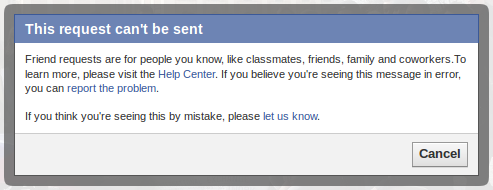
\includegraphics[width=5in]{figures/cantFriend.png}
\caption{Zrušení žádosti o přátelství na facebooku}
\label{fig:cantFriend}
\end{center}
\end{figure}

Během prvního kola přihlašování bylo zasíláno vždy sedm až devět žádostí o nová přátelství. Toto okno se mi zobrazovalo při přidávání většího množství přátel, většinou při více než šesti odelsaných žádostech o přátelství. Ustálil jsem tedy po  tomto zjištění počet přidávaných přátel na pět za~jedno přihlášení.

Počet pěti nových žádostí o přátelství jsem ponechal u každého účtu až do konce experimentu. Pokud se ale stalo, že náš účet obdržel některé žádosti o přátelství od ostatních uživatelů, tak byly všechny přijaty. Počet nově přidaných přátel za jedno přihlášení se pak snižoval o počet přijatých žádostí o přátelství. Pokud počet nových přijatých žádostí o přátelství překročil pět, tak už nebyly posílány další nové pozvánky.

Snažil jsem se, aby nově přidávaní přátelé byli české národnosti. Hlavním důvodem bylo, aby přidané profily rozumněly publikovaným statusům a aby byly požadavky o přátelství realističtější. Při testování první generace se mi stalo, že po přidání několika účtů s arabskými jmény mi facebook začal nabízet pouze arabské přátele. Někteří žádost o přátelství přijali, ale většinou jen ze zvědavosti a daný účet začal dostávat pozvánky na facebookové skupiny s arabskými názvy. Proto jsem se při~experimentu snažil přidávat pouze facebookové uživatele z České republiky.

Pro zachování autentičnosti chování uživatelů facebooku jsem se při přidávání přátel snažil, aby účty zasílaly žádosti o přátelství ve větší míře profilům opačného pohlaví. Tedy aby si experimentální profily se ženským jménem přidávaly více mužských přátel na facebooku a naopak. 

\subsection{Nahrávání statusů k experimentálním účtům na facebooku}

Pro experiment jsem sdílení omezil na přidávání statusů na svou zeď. Jedná se totiž o hlavní možnost, jak dát na facebooku o sobě vědět. Frekvence přidávání statusů byla nastavena na jeden status za přihlášení. 

Obsah vkládaných statusů byl obecný a neutrální. Jednalo se většinou o citáty a výroky známých i neznámých osobností na internetu, vtipy a neutrální a spontánní komentáře aktuálního dění (například o počasí). Jako zdroj pro statusy citátů sloužila webová stránka: \verb|http://citaty.net/| a jako zdroj vtipných statusů sloužily stránky: \verb|http://www.vtipy.net/|, \verb|http://vysmatej.cz/| a \verb|http://vtipy.peoplelovepeople.com/|. Snažil jsem se vyhýbat rasistickým a politickým vtipům, abych nepobouřil některého z přidaných přátel na facebooku. Spontánní texty statusů jsem vymýšlel sám nebo jsem se inspiroval statusy na zdi ostatních účtů.

Mimo klasických textových statusů byly na účty nahrávány i obrázky doplněny textovým popisem. Na facebooku jsou tyto obrázky velmi oblíbené, existují stránky jako \verb|http://9gag.com/| nebo \verb|http://www.rouming.cz/|, které obsahují vtipné obrázky s popisky a facebookoví uživatelé je velmi rádi  sdílejí a dávají jim like. Pro stahován obrázků sloužila především sociální síť instagram. Jako zdroje dalších obrázků pro statusy sloužily obrázky nalezené na ostatních stahovaných profilech nebo na stránkách zmíněných výše. Obzvláště oblíbené jsou v posledních týdnech animované obrázky anebo obrázky doplněné vtipnými texty (takzvané memy).

\subsection{Zajímavosti na které jsem během experimentu narazil}

Po přihlášení k účtu, stažení informací a spuštění automatizovaných akcí jsem vždy ručně kontroloval, co se na facebookovém účtu děje. Ve většině případů se u účtu zobrazovaly notifikace o potvrzení žádostí o~přátelství a několik zpráv od přidávaných profilů, zda náš účet zná osobu, které byla odeslána žádost o přátelství a občas i šťouchnutí.

Facebookové zprávy nebyly automaticky zpracovávány. Zpracovávání by totiž nepřinášelo přidanou hodnotu k našemu experimentu a zpracování textu by bylo složité. Na žádné zprávy jsem nikdy neodpovídal. Teoreticky by bylo možné připravit univerzální odpověď na otázku, zda se dané facebookové účty znají. Například vymyšlení univerzálního místa, kde se mohly dané osoby setkat - škola, práce, apod., anebo přiznání, že se účty neznají. 

Pak by ale zcela určitě pokračovalo další dotazování pomocí facebookových zpráv, odkud se dané účty znají anebo proč byla odeslána žádost o přátelství na facebooku. Nejen, že by takovéto zpracování zabralo mnoho času a~nebylo by možné plně automatizovat, ale někdy by mohlo takovéto chování být i kontraproduktivní.

Při procházení profilů jsem ale občas narazil na zajímavé jevy. Pokud účet neměl na facebooku vyplněné některé informace, konkrétně školu nebo bydliště. Zobrazilo se na facebooku na výpisu zdi (což je stránka, která se zobrazí ihned po přihlášení) nad výpisem statusů upozornění o doplnění těchto informací i s nabídkami. Příklad takovéhoto formuláře je vidět na~obrázku \ref{fig:completeSchool}.

\begin{figure}[h]
\begin{center}
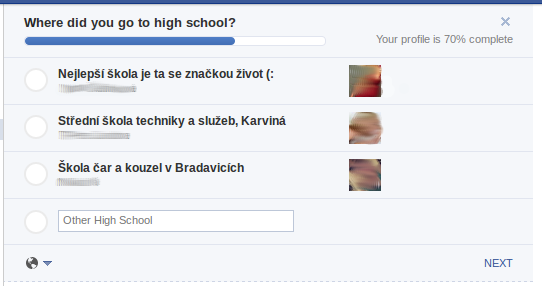
\includegraphics[width=5in]{figures/completeSchool.png}
\caption{Formulář na facebooku nabádající k vyplnění vystudované střední školy}
\label{fig:completeSchool}
\end{center}
\end{figure}

Kromě přidaných formulářů na stránce zdi se po přihlášení u některých účtů zobrazil tříkrokový průvodce pro vyplnění bezpečnostích informací. Jedná se o zadání kontaktních informací při ztrátě facebookového hesla nebo při odcizení facebookového účtu cizí osobou (například při prozrazení hesla k účtu). Pokud by bylo potřeba, facebook umožňuje resetovat heslo a zaslat nové na jeden ze zadaných kontaktních údajů. Jedná se také o ověření, že bude heslo změněno jen skutečným vlastníkem účtu. Zadávají se tyto informace: e-mail, telefonní číslo a bezpečnostní otázka včetně odpovědi. 

Mezi další formuláře pro doplnění informací na facebooku patří možnost výběru URL adresy facebookového profilu. Jde o jednoznačný identifikátor každého uživatele. Adresa profilu pak vypadá následujícím způsobem: \verb|http://www.facebook.com/jan.novak|. Tento identifikátor se používá i pro e-mailovou adresu na facebooku, kterou má každý účet. Například: \verb|jan.novak@facebook.com|. Jakékoli zprávy odeslané na tuto e-mailovou adresu se zobrazí mezi zprávami na facebooku. Pokud si uživatel žádný identifikátor nevybere, získá adresu vygenerovanou od facebooku spojením jména příjmení a náhodného čísla, například: \verb|jan.novak.145|.

Občas se u některých elementů na facebooku objeví malé vyskakovací okno s nápovědou, která popisuje možnosti elementů na facebooku. Jedná se například o oznámení, že lze na facebook nahrávat fotky a odkazy pouhým přetažením do textového pole pro zadávání statusů a podobně. 

U jednoho experimentálního účtu se mi po šestém přihlášení  objevilo okno s oznámením, že byly z tohoto účtu zasílány žádosti o přátelství lidem, které daný účet nezná. Pravděpodobně došlo k tomu, že většina zaslaných pozvánek na facebooku byla zamítnuta a lidé nepotvrdili, že by daný účet znali i v reálném životě. Facebook v tomto okně radí přidávat si lidi, jako jsou: rodinní příslušníci, spolužáci nebo spolupracovníci a lidi, které známe z reálu. Je potřeba odškrtnout potvrzení, že již nebudou rozesílány žádosti o~přátelství lidem, které neznáme z reálného života, jinak může být daný účet zablokován.

Na další obrazovce se objevil seznam zaslaných nepřijatých a nepotvrzených žádostí o přátelství s možností jakékoli žádosti zrušit (jak je vidět na obrázku \ref{fig:cancelPendingFrinedRequests}).

\begin{figure}[h]
\begin{center}
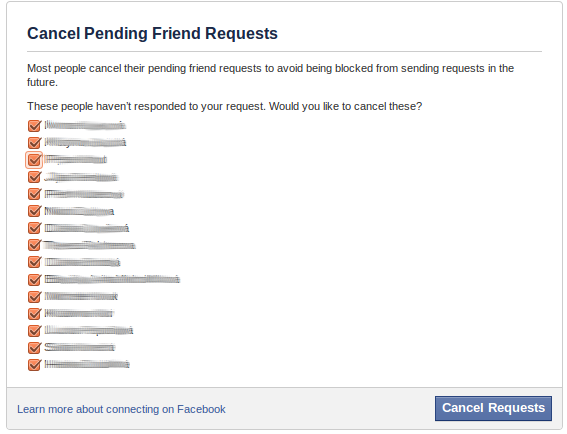
\includegraphics[width=5in]{figures/cancelPendingFriendRequests.png}
\caption{Formulář na facebooku pro zrušení nepřijatých  a nepotvrzených žádostí o přátelství}
\label{fig:cancelPendingFrinedRequests}
\end{center}
\end{figure}

Zrušil jsem tedy všechny tyto žádosti a zaslal jsem pět nových žádostí jako u každého experimentálního účtu. Při příštím přihlášení se mi zobrazil formulář s nutností opsat kontrolní kód a na další obrazovce se objevilo oznámení o zablokování účtu s formulářem pro zadání telefonního čísla (naprosto stejný jako při zakládání více účtů ze stejné IP adresy).

Pravděpodobně došlo odebráním čekajících žádostí o přátelství a ke snížení důvěryhodnosti profilu, jelikož účet obsahoval málo přátel na facebooku. V~době posledního přihlášení před zablokováním obsahoval účet osm potvrzených přátel. Z nichž někteří si mohli do dalšího přihlášení tento účet odebrat. Tím došlo k zablokování daného profilu po 22 dnech od spuštění experimentu. 

Po zablokování jsem se pokoušel k účtu prihlásit vždy po čtyřech dnech, při každém dalším přihlášení, ale vždy jsem byl ihned přesměrován na stejnou obrazovku pro zadání telefonního čísla. Otázkou zůstává, zda by došlo k zablokování profilu i bez~smazání žádostí o přátelství. Pravděpodobně došlo k překročení limitu nepřijatých žádostí o přátelství anebo poměru přijatých a nepřijatých přátelství a facebook zobrazuje tato okna, aby uživatelé nezasílali pozvánky účtům, které o to nestojí.

U jedné odeslané žádosti o přátelství se mi podařilo narazit na další omezení facebooku. Maximální počet přátel, které může každý účet na facebooku mít je pět tisíc. S tím se pojí další limit, jeden účet může mít na~facebooku maximálně jeden tisíc nevyřízených (nezamítnutých nebo nepotvrzených) žádostí o přátelství. Při jedné ze zaslaných žádostí o přidání mezi facebookové přátele se mi zobrazilo vyskakovací okno (viz obrázek \ref{fig:friendRequestsLimitReached}), že kvůli tomuto omezení nebyla žádost o přátelství zaslána. Bohužel s tímto nemůžeme nic udělat, musíme počkat, až účet jemuž byla žádost zaslána tyto nevyřízené žádosti o přátelství potvrdí nebo zamítne.

\begin{figure}[h]
\begin{center}
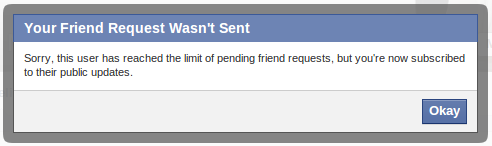
\includegraphics[width=5in]{figures/friendRequestsLimitReached.png}
\caption{Informace o dosažení maximálního počtu nevyřízených žádostí o přátelství na facebooku}
\label{fig:friendRequestsLimitReached}
\end{center}
\end{figure}

K zablokování došlo i u dalšího účtu a to shodně při sedmém přihlašovacím kole, ale nejednalo se o stejný den jako u předchozího profilu. Tentokrát se nezobrazil ani formulář pro zrušení nepřijatých žádostí o přátelství. Ihned po přihlášení jsem byl přesměrován na obrazovku pro zadání kontrolního kódu a následoval formulář pro zadání telefonního čísla.

Během experimentu byly celkem zablokovány pouze tyto dva účty, pokud nepočítám účty zablokované při samotném zakládání. Ostatní účty byly bez problému aktivní až do konce experimentu.

Ve většině případů jsem experimentální účty navštěvoval z~domova, z mé domací IP adresy. Ve dvou dnech jsem se ale připojoval k účtům z jiného místa a IP adresa byla odlišná od mé domácí adresy. Při tomto, v pořadí sedmém, připojování se mi u jednoho z účtů ihned po přihlášení zobrazilo oznámení, že je účet dočasně zablokovaný. Po pokračování na následující obrazovku se mi zobrazil formulář pro ověření identity. Celý formulář je k~vidění na obrázku \ref{fig:confirmIdentity}.

Formulář obsahoval pole pro zadání data narození daného profilu. Naštěstí jsem měl pro každý experimentální účet poznamenané datum narození, které bylo vyplněno při registraci. Po zadání správného data narození už byl účet odblokovaný a bez jakýchkoli omezení. 

Jak je na obrázku formuláře vidět, dočasné zablokování bylo pravděpodobně způsobeno přihlašováním k facebooku z jiné IP adresy. Pod formulářem je napsáno, že pro odblokování účtu se lze místo zadávání data narození přihlásit ze zařízení (IP adresy), ze kterého se daný účet přihlašoval naposledy. Od té doby jsem se přihlašoval už jen pouze z jedné IP adresy.

\begin{figure}[h]
\begin{center}
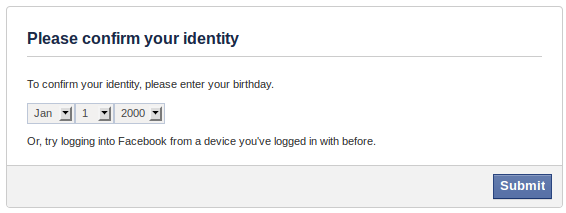
\includegraphics[width=5in]{figures/confirmIdentity.png}
\caption{Formulář pro ověření totožnosti zadáním data narození na~facebooku}
\label{fig:confirmIdentity}
\end{center}
\end{figure}

Při vývoji aplikace jsem používal program Selenium WebDriver k ovládání webového prohlížeče. Při přidávání like ke~statusům na zdi jsem vždy musel stáhnout nejnovější statusy a zjistit, kolik mají jednotlivé příspěvky uděleno like. Po stažení všech příspěvků a vyhodnocení, které mají nejvíce like jsem používal Selenium WebDriver k okamžitému udělení like k vybraným statusům. 

Při programování aplikace jsem ale jednou omylem vložil část pro udělování like ke statusům, což bylo v internetovém prohlížeči realizováno klikem na tlačítko, do špatné sekce v programu. Klik na tlačítko pro udělení like se kvůli tomuto omylu opakoval vždy několikanásobně v rychlém sledu za~sebou.

\begin{figure}[h]
\begin{center}
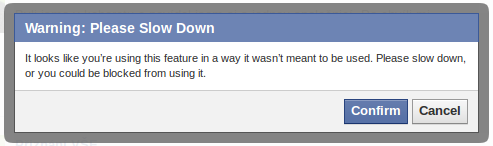
\includegraphics[width=5in]{figures/slowDown.png}
\caption{Facebookové upozornění kvůli příliš rychlé interakci}
\label{fig:slowDown}
\end{center}
\end{figure}

Facebook mi kvůli těmto rychlým interakcím zobrazil upozornění, které je vidět na obrázku \ref{fig:slowDown}. Jednalo se o upozornění, že se děje něco, k čemu by docházet nemělo a že může dojít i k zablokování facebookového účtu. Při~experimentu jsem si na tento problém již dával pozor a mezi interakcemi jsem dělal prodlevy, aby facebook nemohl odhalit automatizaci interakce. Později jsem na toto upozornění již nenarazil.

Nejzajímavější zjištění pro mne nastalo při návštěvě jednoho z profilů v průběhu experimentu. Zjistil jsem totiž, že od posledního navštívení profilu, získal jeden z účtů 48 nových žádostí o přátelství a to při šestém přihlášení od začátku experimentu. Takovéto množství přidaných přátel jsem v žádném případě na začátku experimentu nepředpokládal.

Konkrétně se jednalo o profil se skupinou vyplněnosti 4 a se strategií přidávání profilů s velkým množstvím přátel. Zajímavé na všem bylo, že celkový dosavadní počet přátel profilu byl 18 uživatelů. Jedná se tedy o téměř trojnásobné navýšení počtu přátel. Je nutné dodat že naprostá většina těchto žádostí o přátelství pocházela od profilů mužů na facebooku (pouze jeden byl od ženského profilu).

Profily, které tomuto experimentálnímu účtu zaslaly pozvánku byly z~různých států světa (USA, Egypt, Thajsko a další). Účty byly velmi různorodé, některé vypadaly na první pohled jako falešné účty vytvořené pouze za účelem přidávání přátel, ale některé profily byly naopak velmi vyplněné a obsahovaly autentické fotografie jedné osoby s několikaletou historíí celého profilu, takže se pravděpodobně nejednalo o falešné účty. Nikdy to ale nelze zcela jistě určit. 

S největší pravděpodobností facebook tento profil vyhodnotil jako zajímavý pro ostatní uživatele, tím že si ho přidávali na facebooku vlivné osoby (profily s velkým počtem uživatelů). Díky tomu mohl facebook tento experimentální účet doporučovat pro přátelení s ostatními profily a tak mohl získat velké množství žádsotí o přátelství.

Dalším faktorem tohoto jevu mohla být poměrně pěkná profilová fotka experimentálního účtu. Je možné, že se odkaz na tento facebookový profil objevil na některé internetové stránce a díky tomu si tento profil přidávali ostatní uživatelé. Na facebooku bohužel není žádná možnost zjištění kolik lidí navštíví facebookový profil a odkud uživatele přicházejí.

Další možností k tomuto rozšíření experimentálního profilu mezi další facebookové uživatele, která mne napadá, je možnost doporučení přátel. Facebook po spřátelení dvou profilů dává každému možnost doporučit novému profilu někoho ze svých přátel. Těmto účtům pak přijde upozornění, že jim byl doporučen facebookový  účet k přidání mezi své přátele. Uživatel pak může tomuto účtu poslat žádost o přátelství anebo toto doporučení zamítnout. 

Je tedy pravděpodobné, že jsem požádal o přátelství velmi aktivní profil anebo facebookový účet, který slouží pro získávání co největšího množství přátel. Mohlo by se jednat i o síť vzájemně propojených účtů, které si navzájem doporučují přidané přátele. Jeden takovýto vlivný účet pak mohl náš profil doporučovat ostatním a tím vznikl takto vysoký počet žádostí o~přátelství.

Při dalším přihlášení, tedy po čtyřech dnech měl tento účet dalších 28 nových žádostí o přátelství, což je méně než v předchozím případě. Ale následující přihlášení se u stejného účtu objevilo 71 nových žádostí a u posledního přihlášení dokonce 115 nových žádostí o přátalství. Toto číslo je obrovské, především když si uvědomíme, že medián počtu přátel u~účtů na facebooku je 229 \cite{web:fbFriendsMedian}. Tento jev tedy nebyl náhodný, ale tendence přidávání přátel k tomuto účtu se časem ještě zvyšovala.

Jak k takovému vysokému nárůstu přátel mohlo dojít asi nepůjde dostupnými prostředky nikdy stoprocentně zjistit. S největší pravděpodobností půjde o kombinaci výše zmíněných faktorů na facebooku a možná i~mimo něj.

\section{Vyhodnocení celého experimentu}

Za dobu kterou experiment běžel jsem získal velmi zajímavá data. Zaznamenával jsem především celkový počet uživatelů u jednotlivých účtů. Všechna data jsou zobrazena v tabulkách \ref{tab:friendsCount}, \ref{tab:friendRequestsCount} v příloze. Zaznamenaná data jsou seřazena podle pořadí jednotlivých přihlášení.

Celkový počet přidaných přátel pro jednotlivé účty jsem rozdělil podle pohlaví, jednotlivých strategií přidávání prvních přátel a podle stupně vyplněnosti profilů. Graf přátel pro účty rozdělené podle jednotlivých pohlaví je na grafu \ref{fig:gender}. 

Jak je vidět, ženské profily měly mnohem více přátel než mužské. Jednak to bylo dáno tím, že profil s rekordním počtem přátel byl ženského jména. Za druhé je také potřeba podotknout, že ženských profiů bylo celkově 14 a mužských pouze 11. Jak je vidět z grafu, celkový počet přátel s časem neustále rostl a to i přesto, že některé profily si experimentální účty z přátel odebíraly. 

\begin{figure}[h]
\begin{center}
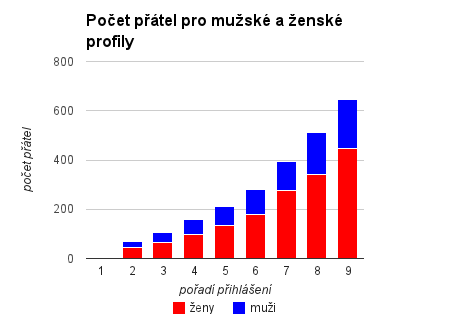
\includegraphics[width=5in]{figures/gender.png}
\caption{Počet přátel pro mužské a ženské profily}
\label{fig:gender}
\end{center}
\end{figure}

Počty přátel u jednotlivých účtů jsem rozdělil podle strategií přidávání prvních přátel. Nejzajímavější z grafů byl se strategií (viz graf \ref{fig:levelMutual}). Sem patřil účet s nejvíce přáteli a zároveň i účet, který byl během experimentu zablokován. Jedná se tedy o velmi různorodou skupinu účtů. 

Ostatní grafy rozdělení účtů podle skupin již nejsou natolik zajímavé. Všechny jsou k dispozici na prostudování v příloze \ref{fig:levelFake}, \ref{fig:levelMany}, \ref{fig:levelGroup} a \ref{fig:levelFb}. Jednotlivé účty jsou u všech grafů rozlišeny podle stupně vyplněnosti profilu.

\begin{figure}[h]
\begin{center}
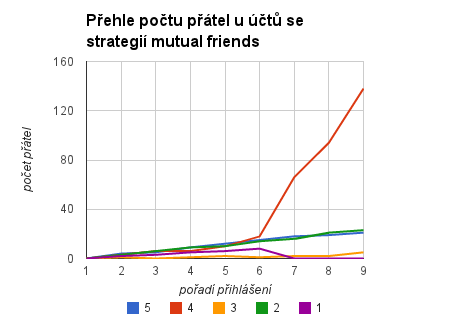
\includegraphics[width=5in]{figures/levelMutual.png}
\caption{Počet přátel pro profily se strategií přidávání prvních přátel mutual friends}
\label{fig:levelMutual}
\end{center}
\end{figure}


Druhým typem rozdělení skupin účtů bylo podle stupně vyplněnosti profilu na stupnici od 1 do 5. Nejzajímavějším grafem podle tohoto rozdělení je se stupněm 4, kde je znovu vidět účet s nejvíce přáteli, jak lze zpozorovat na obrázku \ref{fig:level4}. 

\begin{figure}[h]
\begin{center}
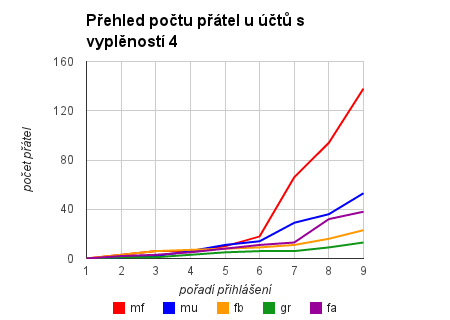
\includegraphics[width=5in]{figures/level4.png}
\caption{Počet přátel pro profily se skupinou vyplněnosti 4}
\label{fig:level4}
\end{center}
\end{figure}

Naopak ze skupiny profilů se stupněm vyplněnosti byly dva z pěti účtů během experimentu zablokovány. K účtům se mi po zablokování již nepodařilo přihlásit, takže je u nich při dalších přihlášeních uvedeno 0 přátel. Zajímavé je, že i přes tento úbytek přátel celkový graf počtu přátel stále stoupá. Celý graf je k vidění v příloze na obrázku \ref{fig:level1}.

Účty jsou na všech grafech rozděleny podle strategie přidávání prvních přátel, takto: mf = many friends, mu = mutual friends, gr = facebook groups, fb = facebook suggestions a fa = fake profiles. Všechny ostatní grafy jsou k vidění v příloze, viz \ref{fig:level5}, \ref{fig:level3} a \ref{fig:level2}.


Ze získaných dat jsem kromě počtu přátel zanalyzoval i data stažených statusů. Za celý experiment se mi podařilo uložit celkem 26~582 statusů na facebooku. Jednalo se o statusy z uživatelských profilů a zdí experimentálních účtů. Některé statusy tedy byly v databázi uloženy vícekrát, protže byly staženy z různých zdrojů.

Jako nejzajímavější mi přišlo rozložení času vkládání jednotlivých statusů v týdnu. Připravil jsem graf znázorňující počet statusů v jednotlivých dnech \ref{fig:postedDays}. Zajímavé je, že nejvíce statusů ze stažených dat bylo vloženo v pondělí a postupem týdne počet vkládaných statusů klesal. Nejméně statusů pak bylo napsáno na facebook ve čtvrtek a pátek.

Jako další jsem připravil graf rozložení času vkládaných statusů podle hodin. Výsledný graf je na obrázku \ref{fig:postedHours}. Jak by se dalo předpokládat, nejvíce statusů bylo na facebook vloženo mezi 19 a 22 hodinou. Nejméně pak v nočních hodinách mezi 0 a 8 hodinou.



Největším překvapením celého experimentu bylo množství obdržených žádostí o přátelství. Celkem za celý experiment získaly všechny účty 470 žádostí o přátelství. Z toho více než polovinu těchto žádostí, konkrétně 274, získal jediný z profilů. 

Před začátkem experimentu jsem nepředpokládal, že by mohly experimentálním účtům chodit žádosti o přátelství. Otázkou zůstává, čím to mohlo být způsobeno. Důležité je zjištění, že pokud se účtu podaří získat žádosti o přátelství, tak při příštím přihlášení s největší pravděpodobností obdrží další žádosti o přátalství.

Na konci experimentu měli všechny aktivní účty 645 přátel, což je poměrně vysoké číslo na to, že experiment běžel po dobu jednoho měsíce. Pro většinu účtů měl postupný růst přátel exponenciální trend. Dalo by se to vysvětlit tak, že účty s narůstajícím počtem přátel získávaly vyšší důvěryhodnost a více účtů bylo ochotných si je přidat mezi své přátele. Celkový počet přijatých žádostí o přátelství ale bude ještě vyšší, jelikož některé účty si během experimentu odebíraly experimentální profily ze svých přátel. 

Nejdůležitější bylo vždy nabrat určitý počet přátel, přibližně kolem deseti až dvaceti. Poté se začal počet přátel zvyšovat rychleji. Pravděpodobně bylo potřeba překonat určitou hranici důvěryhodnosti pro ostatní účty na facebooku. Průměrný počet přátel pro aktivní účty je 28 a medián je 22. 

Někteří facebookoví uživatelé si experimentální účty přidali jen aby zjistili, zda náhodou daný účet neznají a po čase přátelství zrušili. Odliv přátel nebyl nijak extrémní, většinou se jednalo pouze o jednotky uživatelů. 

Z pětadvaceti účtů, se kterými jsem na začátku experiment začínal zbylo na konci 23 aktivních účtů. Dva z účtů byly zablokovány. Jednalo se o účty, jejichž počet přátel byl při posledním přihlášení před zablokováním 8 a 9. Některé účty měly po celou dobu experimentu nižší počet přátel a přesto zablokované nebyly.

S největší pravděpodobností se jednalo o nahlášení ze strany uživatelů. Pokud komukoliv příjde na facebooku žádost o přátelství od účtu, který nezná, má možnost označit dotyčný účet jako nepravý. Pokud facebooku příjde více takových stížností, tak účet pravděpodobně zablokuje, stejně jako tomu bylo v našem případě. Možná to bude mít spojitost s tím, že oba účty patřily do skupiny vyplněnosti se stupněm jedna, to znamená, že neměly vyplněné žádné informace o dané osobě.

Při zablokování účtu se zobrazí nejprve kontrolní formulář pro opsání textu z obrázku, aby facebook odfiltroval automatické roboty a poté se zobrazí formulář pro zadání telefonního čísla na které příjde ověřovací kód. Přejít přes tento krok je velmi složité, jelikož telefonní číslo se oproti například e-mailu nedá jednoduše získat a ve většině zemí je k získání telefonního čísla potřeba smlouva s telekomunikačním operátorem.


Pokud se zaměříme na profily podle jednotlivých skupin vyplněnosti, můžeme vidět, že nejvíce přátel má skupina se stupněm 4. V této skupině je účet, který získal rekordní počet žádostí o přátelství, ale i bez tohoto účtu by měla tato skupina nejvíce přátel. Mezi skupinami se stupněm 3 a 5 není extra velký rozdíl v počtu přátel a skupina se stupněm 2 je za nimi. Nejméně přátel má pak podle očekávání skupina se stupněm 1, tedy účty, které o sobě neměly vyplněné žádné informace, dva z účtů byly zablokovány, ale i u ostatních byl počet přátel podprůměrný.


Pokud se zaměříme na jednotlivé strategie pro přidávání různých skupin prvních přátel na facebooku, tak můžeme vidět, že nejvíce přátel získala strategie many friends. Ale to jen díky tomu, že do této skupiny patřil účet s velkým množstvím žádostí od ostatních. Kromě tohoto účtu byl počet přátel v této skupině podprůměrný. Druhou nejúspěšnější strategií bylo mutual friends, pravděpodobně se to dá vysvětlit tím, že uživatelé jsou více ochotní přidávat si účty, které již mají v přátelích někoho z jejich přátel na facebooku.

Jako třetí v pořadí je strategie, která spoléhá na přidávání falešných účtů. Pravděpodobně to bude záviset na tom, že některé falešné účty jsou vytvořeny za účelem získávání výhod ve hrách na facebooku anebo pro přidání některého z přátel na facebooku bez prozrazení pravé identity. Takovéto falešné účty pak nemají motivaci přidávat si nové přátele.

Předposlední strategií v počtu přidaných přátel je facebook groups. A~jako strategie s nejmenším počtem přidaných přátel se stala skupina facebook suggestions. 

Výsledky těchto statistik jsou ovlivněny mnoha faktory na facebooku. Pro přidávání přátel na facebooku nejvíce záleží na účtech, které si přidáváme. Některé účty mohou být velmi aktivní a sami nám mohou doporučovat své přátele a také náš účet svým přátelům. 

U ostatních účtů, které nejsou příliš aktivní poté záleží především na důvěryhodnosti přidaného účtů. Profilová a úvodní fotka na facebooku proto hrají velmi důležitou roli. Profily bez fotek a s málo informacemi byly zablokovány a měly méně přátel. Pokud ale profil překročí vyplněností určitou mez, tak už není třeba přidávat o profilu další informace, jak bylo patrné u skupin vyplněnosti.

Počet uživatelů u experimentálních účtů by šel pravděpodobně celkově zvýšit přidáváním více přátel při každém přihlášení. Mohlo by ale dojít k vyššímu počtu zablokovaných účtů, pokud by velké množství přidaných profilů nahlásilo účty jako  falešné.

Druhým způsobem, jakým by šel zvýšit celkový počet přátel by bylo častější přihlašování k profilům. Tím pádem by bylo za stejný časový úsek odesláno větší množství žádostí o přátelství a byla by zvýšena celková aktivita profilu.


%\begin{conclusion}
%\end{conclusion}
\chapter{Z{\' a}v{\v e}r}

Před začátkem experimentu jsem si nebyl jistý, jak se budou ostatní facebookové účty chovat k experimentálním profilům a na jaké zádrhele mohu narazit. Při běhu experimentu mne nejvíce překvapilo množství přijatých žádostí od zcela neznámých profilů.

\section{Shrnutí experimentu}

Při experimentu, kdy nebyla zvolena příliš agrasivní strategie přidávání přátel se podařilo během jednoho měsíce u 23 aktivních účtů nasbírat 645 přátel. Přičemž se k jednotlivým účtům přihlašovalo jednou za 4 dny a bylo zasíláno pět žádostí o přátelství při každém přihlášení. Určitě by bylo zajímavé sledovat experiment po delší dobu, kde by se počet přidávaných přátel zastavil a kolik by bylo možné získat dohromady přátel na facebooku za delší období.

Dva z pětadvaceti účtů byly zablokovány, jednalo se o účty bez profilové fotky a s nízkým počtem přátel, pod deset v době zablokování. Pravděpodobně by šlo zablokování profilů zabránit vyplněním více informací o účtu a přidáním fotek. Možná by také pomohlo přidávát zpočátku experimentu k účtům více přátel, aby experimentální profily nasbíraly více jak deset přátel a zvýšila by se tím jejich věrohodnost. Otázkou zůstává, zda by facebook přidávání většího množství přátel toleroval a aby takovéto počínání nevedlo naopak k rychlejšímu zablokování účtů.

Podle získaných zkušeností z provedeného experimentu jsem zjistil, že pro přidávání velkého počtu přátel na facebooku jsou důležité následující parametry. Jedná se především o pěknou profilovou fotku a to ženského pohlaví. Ženské profily měly vyšší úspěšnost. Poté je důležité, aby profil získal určitou důvěryhodnost. Toho se dá dosáhnout především vyplněním informací o profilu a získáním určitého množství přátel, jednalo se většinou o počet kolem deseti až dvaceti.


\section{Možné způsoby rozšíření a pokračování v experimentu}

Při provádění experimentu mne napadlo několik možných směrů, jak by šlo vše rozšířit a na co by se dalo dále zaměřit.

\subsection{Automatizace zakládání facebookových účtů}

Teoreticky by bylo možné celý proces zakládání facebookových účtů plně zautomatizovat. E-mailové adresy pro registrované účty by šlo jednoduše zařídit na vlastní doméně nastavením doménového koše. To znamená, že veškeré e-maily, které byly odeslané na adresu naší domény budou doručeny na jednu konkrétní e-mailovou adresu. Získáme tak teoreticky neomezené množství e-mailů k registraci na facebook. Otázkou je, zda by facebooku nevadila stejná doména, ale některé firmy a školy vytvářejí pro své zaměstnance a studenty e-mailové adresy s doménou instituce, takže by to nemuselo vadit.

Dále by se musel vyřešit problém s registrací z jedné IP adresy denně. Toto omezení by šlo obejít použitím několika spolehlivých proxy serverů\footnote{Proxy server - server, prostřednictvím kterého se lze připojit k internetu, výhodou je že není vidět naše IP adresa, ale IP adresa proxy serveru, seznam proxy serverů lze nalézt na internetu, například - http://www.hidemyass.com/proxy-list/}, přes které by byly facebookové účty registrovány. Množství registrovaných účtů na facebooku denně by se odvíjelo od počtu využívaných proxy serverů. Čím více, tím lépe.

Pravděpodobně by se musel vyřešit i problém s opisováním kontrolního CAPTCHA kódu, pokud facebook detekuje podezřelou robotickou činnost. Na internetu ale fungují služby, které umí za poplatek řešit opisování CAPTCHA obrázků\footnote{http://decaptchablog.com/decaptcher-services}. Vše funguje automaticky pomocí OCR (Optical character recognition - optické rozpoznávání znaků) anebo lidským opisováním textů. Výhodou takovýchto služeb je, že si lze vše pronajmout a~nemusíme se starat o nic jiného. 

Na druhou stranu, by se ani problém s nutností řešit opisování kontrolních kódů z obrázků řešit nemusel. Ve většině případů totiž po zobrazení stránky s opsáním kontrolního CAPTCHA kódu následovala stránka s nutností zadat telefonní číslo a přes tento krok by bylo příliš složité se hromadně dostávat.

Pravděpodobně by bylo potřeba řešit i jiné problémy spojené s automatickým zakládáním facebookových profilů, které by se objevily při hlubším bádání nad problémem. Každopádně se ale určitě jedná o velmi zajímavé téma, které by šlo zpracovat více do hloubky. Protože by rozsah takovéhoto rozpracování pravděpodobně vydal na samostatnou diplomovou práci. Pro~svůj experiment jsem potřeboval pouze omezený počet facebookových účtů, takže jsem všechny účty zakládal ručně.

\section{Rozpoznávání textu facebookových statusů a komentářů}

Pro naši aplikaci nebylo potřeba uchovávat texty komentářů, jelikož jsme sledovali pouze počet komentářů a like u statusů. Ukládal se pouze počet komentářů, který lze získat zpracováním zobrazeného textu. Ukládání textu komentářů by mohlo být užitečné, pokud by bylo možné zjistit citové zabarvení komentářů a statusů (negativní/pozitivní/neutrální). Pro takovéto analýzy jsou ale potřeba pokročilé algoritmy pro práci s textem a pro kvalitní rozpoznání by bylo potřeba delší úseky textů. Takovéto analýzy se využívají pro sledování nálady ve~společnosti (například při volbách apod.) anebo pro sledování spokojenosti s určitým produktem nebo značkou na sociálních sítích. 

Hlavní cíl experimentu byl ale odlišný a počet facebookových účtů, které byly do experimentu zahrnuty nebyl dostatečně velký (hlavně počet facebookových přátel účtů), aby měly výsledky vypovídající hodnotu. Každopádně by se při větším množství účtů zahrnutých do experimentu a při striktním zacílení na uživatele z jedné země mohlo podařit získat vypovídající masu lidí, kde by mohly být výsledky zajímavé. Zatím jsou takováto data získávána pouze z veřejně dostupných zdrojů anebo ze stránek na facebooku a takováto data mohou být zkreslená (omezením vzorku jen na určitou skupinu uživatelů). Jedná se o jeden ze~směrů, kterým by se dal experiment dále rozšířit a pokračovat v~něm v budoucnu.

Kromě získávání nálady ve společnosti by bylo možné i ovlivňovat ostatní profily. Vkládáním pozitivních statusů o určitém příspěvku by mohlo sloužit jako zajímavá reklama. Lidé jsou odmítaví ke klasickým formám reklamy (letáky, televizní reklamy, apod.), ale pokud by se jednalo o pozitivně laděné sdělení, které by nevypadalo na první pohled jako reklama, mohlo by se jednat o zajímavou možnost ovlivnit mínění facebookových uživatelů. Teoreticky by nemuselo být sdělení pozitivní, někdy by mohla stačit zmínka na facebooku a uživatelé by se díky sociální aktivitě (sdílení, dávání like a komentování) postarali o šíření mezi další uživatele internetu. Reklama by teoreticky mohla být i negativní a bylo by zajímavé porovnávat, zda by se více šířily pozitivní nebo negativní statusy. V dnešní době už existují služby pro placené blogové články na míru (Například \verb|http://placla.cz/|). Podobně by to mohlo fungovat i u facebooku.

Facebook na podzim roku 2012 zavedl možnost placení za zviditelnění statusů. Na facebooku se nyní nezobrazují všechny statusy od vašich přátel, ale jen vybrané statusy, které facebook považuje pro vás za nejhodnotnější a nejkvalitnější. Vše jde nastavit a ovlivnit skupinami do kterých si přátele zařadíte. Algoritmy pro zobrazování příspěvků bohužel nejsou veřejné. Nikdy ale nemáte jistotu, že váš příspěvek uvidí všichni (nebo určití) přátelé. Za~poplatek \$6.99 (přibližně 140 Kč - duben 2013) pak uživaté facebooku mohou zviditelnit své příspěvky, aby se zobrazily většímu počtu kamarádů. Takto lze promovat příspěvky i u facebookových stránek, kde tato funkce dává větší smysl.




\bibliographystyle{csn690}
\bibliography{mybibliographyfile}

\appendix

\chapter{Tabulky a grafy dat z experimentu}


\begin{figure}[h]
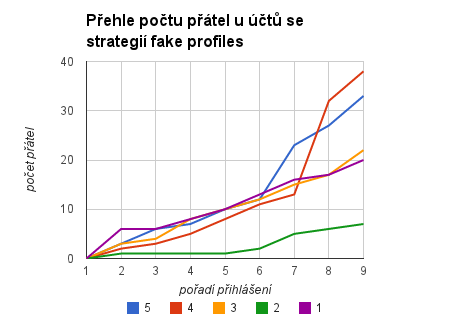
\includegraphics[width=5in]{figures/levelFake.png}
\caption{Počet přátel pro profily se strategií fake profiles}
\label{fig:levelFake}
\end{figure}

\begin{figure}[h]
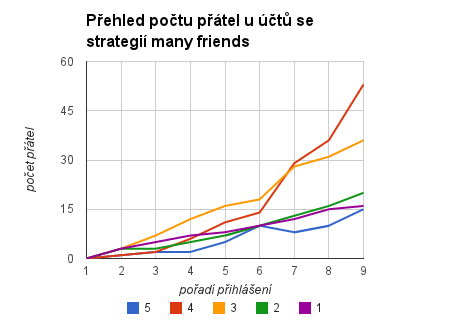
\includegraphics[width=5in]{figures/levelMany.png}
\caption{Počet přátel pro profily se strategií many friends}
\label{fig:levelMany}
\end{figure}

\begin{figure}[h]
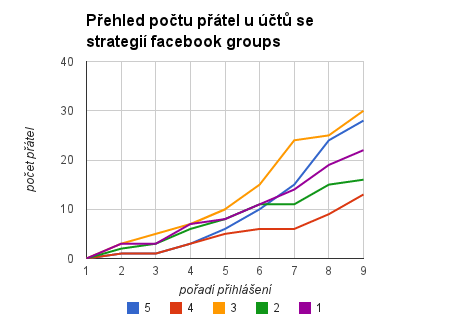
\includegraphics[width=5in]{figures/levelGroup.png}
\caption{Počet přátel pro profily se strategií facebook groups}
\label{fig:levelGroup}
\end{figure}

\begin{figure}[h]
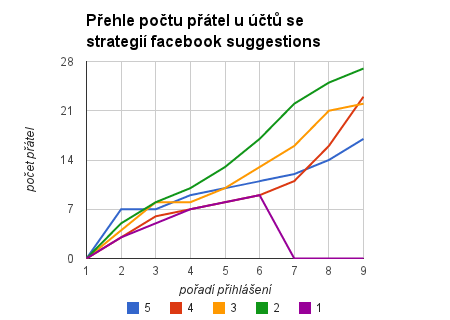
\includegraphics[width=5in]{figures/levelFb.png}
\caption{Počet přátel pro profily se strategií facebook suggestions}
\label{fig:levelFb}
\end{figure}

\begin{figure}[h]
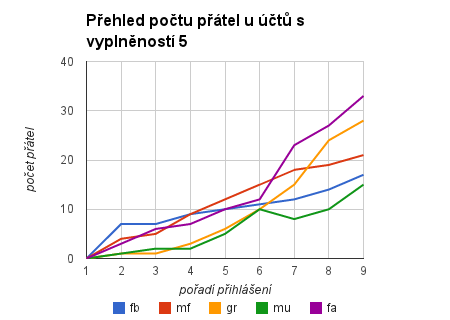
\includegraphics[width=5in]{figures/level5.png}
\caption{Počet přátel pro profily se skupinou vyplněnosti 5}
\label{fig:level5}
\end{figure}

\begin{figure}[h]
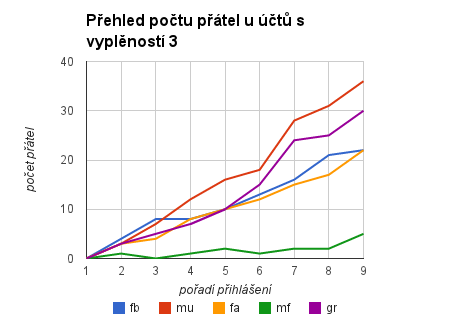
\includegraphics[width=5in]{figures/level3.png}
\caption{Počet přátel pro profily se skupinou vyplněnosti 3}
\label{fig:level3}
\end{figure}

\begin{figure}[h]
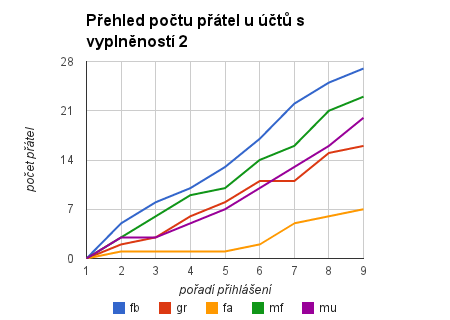
\includegraphics[width=5in]{figures/level2.png}
\caption{Počet přátel pro profily se skupinou vyplněnosti 2}
\label{fig:level2}
\end{figure}

\begin{figure}[h]
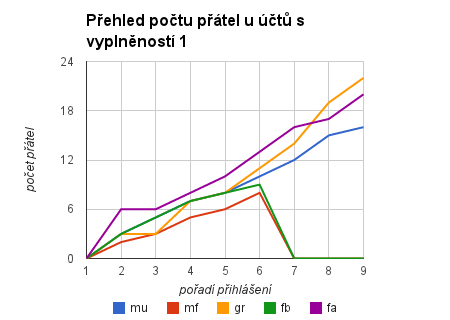
\includegraphics[width=5in]{figures/level1.png}
\caption{Počet přátel pro profily se skupinou vyplněnosti 1}
\label{fig:level1}
\end{figure}

\begin{figure}[h]
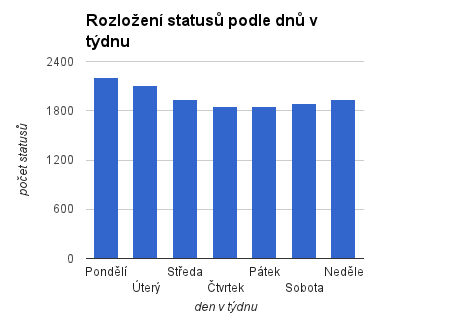
\includegraphics[width=5in]{figures/postedDays.png}
\caption{Rozložení statusů podle dnů v týdnu}
\label{fig:postedDays}
\end{figure}

\begin{figure}[h]
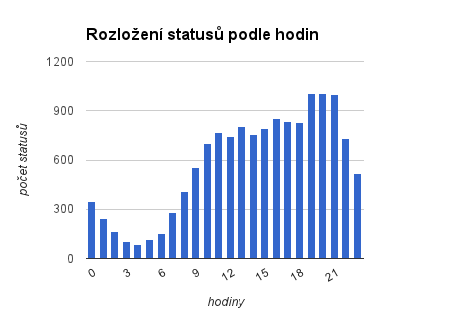
\includegraphics[width=5in]{figures/postedHours.png}
\caption{Rozložení statusů podle hodin}
\label{fig:postedHours}
\end{figure}


\begin{table}[h]
	\centering
	\caption{Vývoj počtu přátel u jednotlivých experimentálních účtů při jednotlivých přihášeních}\label{tab:friendsCount}
	Účty jsou rozděleny podle vyplněnosti profilu (vypl), strategie přidávání přátel (stra) a pohlaví (pohl). Sloupce v tabulce znázorňují jednotlivá přihlášení k účtům. Účty s nulovým počtem přátel ve sloupcích 7 až 9 byly při sedmém přihlášení zablokovány.
	
    \begin{tabular}{ccc | ccccccccc}
    \textbf{vypl} & \textbf{stra} & \textbf{pohl} & \textbf{1} & \textbf{2} & \textbf{3} & \textbf{4}  & \textbf{5} & \textbf{6}  & \textbf{7}  & \textbf{8}  & \textbf{9}   \\ \hline
    5          & fb        & Z       & 0 & 7 & 7 & 9  & 10 & 11 & 12 & 14 & 17  \\
    5          & mf        & M       & 0 & 4 & 5 & 9  & 12 & 15 & 18 & 19 & 21  \\
    5          & gr        & M       & 0 & 1 & 1 & 3  & 6  & 10 & 15 & 24 & 28  \\
    5          & mu        & Z       & 0 & 1 & 2 & 2  & 5  & 10 & 8  & 10 & 15  \\
    5          & fa        & Z       & 0 & 3 & 6 & 7  & 10 & 12 & 23 & 27 & 33  \\
    4          & mf        & Z       & 0 & 3 & 6 & 6  & 10 & 18 & 66 & 94 & 138 \\
    4          & mu        & Z       & 0 & 1 & 2 & 6  & 11 & 14 & 29 & 36 & 53  \\
    4          & fb        & M       & 0 & 3 & 6 & 7  & 8  & 9  & 11 & 16 & 23  \\
    4          & gr        & M       & 0 & 1 & 1 & 3  & 5  & 6  & 6  & 9  & 13  \\
    4          & fa        & M       & 0 & 2 & 3 & 5  & 8  & 11 & 13 & 32 & 38  \\
    3          & fb        & M       & 0 & 4 & 8 & 8  & 10 & 13 & 16 & 21 & 22  \\
    3          & mu        & Z       & 0 & 3 & 7 & 12 & 16 & 18 & 28 & 31 & 36  \\
    3          & fa        & Z       & 0 & 3 & 4 & 8  & 10 & 12 & 15 & 17 & 22  \\
    3          & mf        & M       & 0 & 1 & 0 & 1  & 2  & 1  & 2  & 2  & 5   \\
    3          & gr        & Z       & 0 & 3 & 5 & 7  & 10 & 15 & 24 & 25 & 30  \\
    2          & fb        & M       & 0 & 5 & 8 & 10 & 13 & 17 & 22 & 25 & 27  \\
    2          & gr        & Z       & 0 & 2 & 3 & 6  & 8  & 11 & 11 & 15 & 16  \\
    2          & fa        & M       & 0 & 1 & 1 & 1  & 1  & 2  & 5  & 6  & 7   \\
    2          & mf        & Z       & 0 & 3 & 6 & 9  & 10 & 14 & 16 & 21 & 23  \\
    2          & mu        & Z       & 0 & 3 & 3 & 5  & 7  & 10 & 13 & 16 & 20  \\
    1          & mu        & M       & 0 & 3 & 5 & 7  & 8  & 10 & 12 & 15 & 16  \\
    1          & mf        & M       & 0 & 2 & 3 & 5  & 6  & 8  & 0  & 0  & 0   \\
    1          & gr        & Z       & 0 & 3 & 3 & 7  & 8  & 11 & 14 & 19 & 22  \\
    1          & fb        & Z       & 0 & 3 & 5 & 7  & 8  & 9  & 0  & 0  & 0   \\
    1          & fa        & Z       & 0 & 6 & 6 & 8  & 10 & 13 & 16 & 17 & 20  \\ \hline
               &   & \textbf{součet} & 0 & 71 & 106 & 158 & 212 & 280 & 395 & 511 & 645  \\
    \end{tabular}
\end{table}


\begin{table}[h]
	\centering
	\caption{Vývoj počtu žádostí o přátelství pro jednotlivé profily}\label{tab:friendRequestsCount}
	Účty jsou rozděleny podle vyplněnosti profilu (vypl), strategie přidávání přátel (stra) a pohlaví (pohl). Sloupce v tabulce znázorňují jednotlivá přihlášení k účtům, jako první je v tabulce uvedeno až třetí přihlášení, jelikož v předchozích přihlášeních ani jeden z účtů nezískal žádnou žádost o přátelství.
	
    \begin{tabular}{ccc | ccccccc | c}
    \textbf{vypl} & \textbf{stra} & \textbf{pohl} & \textbf{3} & \textbf{4} & \textbf{5} & \textbf{6} & \textbf{7} & \textbf{8} & \textbf{9} & \textbf{součet} \\ \hline
    5          & fb        & Z       & 0   & 0   & 0   & 0   & 0   & 0   & 1   & 1   \\
    5          & mf        & M       & 1   & 0   & 0   & 0   & 0   & 0   & 0   & 1   \\
    5          & gr        & M       & 0   & 0   & 1   & 1   & 7   & 1   & 0   & 10  \\
    5          & mu        & Z       & 0   & 0   & 0   & 0   & 0   & 0   & 9   & 9   \\
    5          & fa        & Z       & 0   & 0   & 0   & 12  & 0   & 7   & 0   & 19  \\
    4          & mf        & Z       & 0   & 4   & 8   & 48  & 28  & 71  & 115 & 274 \\
    4          & mu        & Z       & 3   & 3   & 1   & 15  & 7   & 17  & 6   & 52  \\
    4          & fb        & M       & 0   & 0   & 0   & 0   & 0   & 2   & 0   & 2   \\
    4          & gr        & M       & 0   & 1   & 0   & 0   & 0   & 0   & 1   & 2   \\
    4          & fa        & M       & 0   & 0   & 1   & 0   & 19  & 10  & 0   & 30  \\
    3          & fb        & M       & 0   & 0   & 0   & 0   & 1   & 1   & 0   & 2   \\
    3          & mu        & Z       & 3   & 1   & 0   & 10  & 0   & 5   & 0   & 19  \\
    3          & fa        & Z       & 0   & 1   & 1   & 1   & 0   & 1   & 0   & 4   \\
    3          & mf        & M       & 0   & 0   & 0   & 0   & 0   & 0   & 0   & 0   \\
    3          & gr        & Z       & 0   & 0   & 4   & 9   & 3   & 7   & 2   & 25  \\
    2          & fb        & M       & 1   & 1   & 1   & 5   & 0   & 1   & 0   & 9   \\
    2          & gr        & Z       & 0   & 1   & 1   & 0   & 0   & 1   & 0   & 3   \\
    2          & fa        & M       & 0   & 0   & 0   & 0   & 0   & 0   & 0   & 0   \\
    2          & mf        & Z       & 0   & 0   & 0   & 0   & 0   & 0   & 0   & 0   \\
    2          & mu        & Z       & 0   & 0   & 0   & 1   & 0   & 4   & 1   & 6   \\
    1          & mu        & M       & 0   & 0   & 0   & 0   & 0   & 0   & 0   & 0   \\
    1          & mf        & M       & 0   & 0   & 0   & 0   & 0   & 0   & 0   & 0   \\
    1          & gr        & Z       & 0   & 0   & 0   & 0   & 0   & 0   & 0   & 0   \\
    1          & fb        & Z       & 0   & 0   & 0   & 0   & 0   & 0   & 0   & 0   \\
    1          & fa        & Z       & 0   & 0   & 1   & 0   & 1   & 0   & 0   & 2   \\
    \end{tabular}
\end{table}



\chapter{Slovník použitých pojmů a zkratek}
%\printglossaries
\begin{description}
	\item[HTML] - Hypertext markup language - zdrojový formát vzhledu webových stránek, který je zpracováván internetovým prohlížečem
		\newline(http://en.wikipedia.org/wiki/HTML).
	\item[Like skupiny na facebooku] - Like = Líbí se mi - způsob připojení se ke~skupně (Group) nebo stránce (Page) na facebooku
	\item[Like statusu] - Like = Líbí se mi - způsob vyjádření, že se uživatelovi líbí status na facebooku, bez nutnosti status komentovat. Jedná se o~modré tlačítko, na kterém je znázorněn palec nahoru.
	\item[Přidat se do vztahu na facebooku] - Na facebooku lze v informacích o~sobě vyplnit i svůj partnerský a rodinný vztah, například: ve volném vztahu, zadaný, v komplikovaném vztahu, ženatý, rozvedený a další. K tomuto stavu můžeme přiřadit i konkrétní osobu s účtem na facebooku, pokud dotyčná osoba vše schválí, zobrazí se pak v informacích odkaz na účet se kterým je osoba ve vztahu.
	\item[Přítel na facebooku] - Jedná se o virtuální kamarádství mezi dvěma lidmi, které funguje tak, že oba zúčastnění musí přátelství potvrdit. Prakticky vše probíhá tak, že můžeme komukoli na facebooku zaslat pozvánku k přátelství, dotyčný pak může pozvánku přijmout anebo odmítnout.  
	\item[Profil na facebooku] - Jedná se o registraci reálného uživatele na facebooku. Lze to přirovnat k virtuální facebookové identitě, může obsahovat různé informace ze života dané osoby. Ostatní uživatelé mohou s daným člověkem komunikovat na facebooku skrze jeho profil.
	\item[(internetový) prohlížeč = browser] - Program pro zpracování a zobrazování internetových stránek. Zpracovává takzvaný HTML kód webové stránky.
	\item[REST] - Representational state transfer - Architektura rozhraní pro komunikaci s webovými službami (Web services), postavený nad HTTP protkolem
\newline(https://en.wikipedia.org/wiki/Representational\_state\_transfer).
	\item[Status] - Příspěvek na svou facebookovou zeď od uživatelů (Facebook nabádá k odpovědi na otázku: „What is on your mind?“ = „Co se vám honí hlavou?“).
	\item[Skupina = stránka na facebooku]
	\item[Šťouchnout na facebooku (Poke)] -
	\item[Zeď na facebooku] - V terminologii facebooku se zeď používá k označení seznamu příspěvků svých a svých kamarádů.
	\item[URL] - Uniform resource locator. Jedná se o adresu webových stránek, která je zobrazena v prohlížeči. Tato adresa identifikuje jednoznačně webové stránky. 
\end{description}

\chapter{Obsah přiloženého CD}

\begin{figure}
	\dirtree{%
		.1 readme.txt\DTcomment{stručný popis obsahu CD}.
		.1 exe\DTcomment{adresář se spustitelnou formou implementace}.
		.1 src.
		.2 impl\DTcomment{zdrojové kódy implementace}.
		.2 thesis\DTcomment{zdrojová forma práce ve formátu \LaTeX{}}.
		.1 text\DTcomment{text práce}.
		.2 thesis.pdf\DTcomment{text práce ve formátu PDF}.
		.2 thesis.ps\DTcomment{text práce ve formátu PS}.
	}
\end{figure}

\end{document}
